\section{Disk matchings and the two-gap cylinder sum}
\label{c2:sec-disk-gluing}

The boundary calculation has given finite masses for collections of disjoint
arcs and the braid identity~\eqref{c2:eq-3}. We now use those arcs to study
polygons on a cylinder. Fix two opposite gaps on a cylinder of circumference
\(2n|U|\), and give each collection of disjoint polygons separating those gaps
its critical vertex weight, with an additional factor \(2\) per polygon.
Our goal is to prove that the total weight is \(n^{1/6+o(1)}\).

The argument has three parts. First we construct a finite vector indexed by
disk matchings, and calculate a twisted pairing of two such vectors. Gluing
the matchings interprets that pairing as the required polygon sum. Next a
contour representation bounds the pairing after its scalar normalization
has been removed. Finally an independent determinant calculation determines
that normalization. Positivity of the polygon sum then makes the upper
bound sharp.

Throughout the disk and contour calculations set
\[
 \lambda=\pi/8,\qquad q=e^{2i\lambda},\qquad
 \mu=2\cos(3\lambda),\qquad d=\sqrt2.
\]
In particular, the letter \(d\) in these sections denotes \(\sqrt2\), rather
than the sine abbreviation used in the boundary calculation.

\subsection{Disk states and their local maps}
\label{c2:sec-disk-states}

Let \(\mathcal D_N\) be the vector space with basis the partial
noncrossing pairings of \(N\) cyclically ordered boundary points of a disk.
A point is either vacant or the endpoint of one arc. Composition joins
arcs at occupied ports and gives weight zero to every closed loop.
Forgetting the filled cylinder end sends each annular state from
Section~\ref{c2:boundary} to such a disk matching. The different annular
states with that matching contribute to the same disk coordinate.

We will check local diagram identities in a faithful spin realization.
At each port use the three-dimensional space with basis \(0,+1,-1\),
where \(0\) means vacancy. An arc with earlier endpoint \(s\) and later
endpoint \(t\) contributes
\[
 \mathsf c_{st}=q^s\delta_{s,-t},\qquad s,t\in\{+1,-1\}.
\]
A matching is the tensor product of these arc coefficients and its vacant
coordinates. The same symbol \(\mathsf c\) denotes the resulting cup
vector or its two-by-two coefficient matrix. Caps use the transpose cup,
without complex conjugation; through-lines preserve spins. Hence
\[
 \mathsf c^t\mathsf c=q^2+q^{-2}=0,
 \qquad \sum_{t=\pm1}\mathsf c_{st}\mathsf c_{tu}=\delta_{su}.
\]
The first identity removes a closed loop; the second straightens a cup
followed by a cap. The boundary constant \(c\) keeps its earlier meaning.

The matching vectors are linearly independent. Fix the occupied sites
and encode a noncrossing matching by its Dyck word: opening endpoints
have spin \(+1\), closing endpoints spin \(-1\). Every spin word with
nonzero coefficient in that matching has partial sums no larger than
those of its Dyck word. The coefficient at the Dyck word is nonzero,
and stack pairing recovers its unique matching. Ordering Dyck words by
partial sums therefore gives a triangular coefficient matrix with
nonzero diagonal. Different occupied sets have disjoint spin support.
For a rectangle, bend its input ports to outputs in reverse order using
nested cups, allowing vacancy with coefficient one at each bend. This
preserves distinct diagrams, so the same argument proves faithfulness
for the local maps used below. A rotation always means rotation of disk
diagrams; its spin realization need not be plain cyclic permutation.

Write \(A(u),B(u),C(u),D(u),E(u)\) for the \emph{normalized} five nonvacant weights, and \(M(u)=T_u\check R(u)\) for the numerator braid. With \(P_w=\sin w,\ b=\sin(2\lambda)\) they are
\[
\begin{aligned}
 T_u&=P_{u+2\lambda}P_{u+3\lambda},&
 A(u)&=\frac{bP_{3\lambda-u}}{T_u},& B(u)&=\frac{bP_u}{T_u},\\
 C(u)&=\frac{P_uP_{3\lambda-u}}{T_u},&
 D(u)&=\frac{P_{2\lambda-u}P_{3\lambda-u}}{T_u},&
 E(u)&=\frac{P_uP_{u-\lambda}}{T_u}.
\end{aligned}
\]
Use rapidities \(z_i\), variables \(x_i=e^{2iz_i}\); an adjacent exchange acting on columns uses \(\check R(z_{i+1}-z_i)\). Half powers of \(x_i\) always mean \(e^{iz_i}\). Unitarity \(\check R(-u)\check R(u)=1\) follows directly (on a single occupied spin use the matrix with diagonal \(A\) and off-diagonal \(C\); on 00 and the doubly occupied space the blocks are \(1,B\mathsf c^t,B\mathsf c,D+E\mathsf c\mathsf c^t\)). Indeed
\[
 A(-u)A(u)+C(-u)C(u)=1,\quad A(-u)C(u)+A(u)C(-u)=0,\quad D(u)D(-u)=1,
\]
\[
 B(u)+B(-u)D(u)=0,\quad D(u)E(-u)+E(u)D(-u)+B(u)B(-u)=0
\]
by angle sums (use \(D(u)=T_{-u}/T_u,\ b^2-P_u^2=P_{2\lambda-u}P_{2\lambda+u},\ P_{u+\lambda}T_{-u}+P_{u-\lambda}T_u=b^2P_u\), the latter by \(T_u=b\sin(3\lambda)+P_u P_{3\lambda-u}\)).

\paragraph{Fusion maps.}
Fusion replaces a special adjacent pair by a single site, or deletes
that pair. On the spin spaces the corresponding insertion maps are
\(J:\mathbb C^3\to(\mathbb C^3)^{\otimes2}\) and
\(K:\mathbb C\to(\mathbb C^3)^{\otimes2}\):
\[
 J0=00+b_0 \mathsf c,\quad Js=b_0(0s+s0),\qquad b_0=(2\cos\lambda)^{-1};\qquad
 K(1)=00+\mathsf c .
\]
Here \(J0\) is the image of a vacancy, while \(Js\) is the image of
an occupied spin. Both maps are injective. The identities we need say
that the braid at the fusion parameter factors through the smaller
space, and that an auxiliary strand can pass the inserted pair:
for \((L,h)=(J,\lambda),(K,3\lambda/2)\), respectively,
\begin{equation}
 \check R(2h)=LL^t,\qquad
 \check R_{12}(u-h)\check R_{23}(u+h)(L\otimes1)=(1\otimes L)R_f,
 \quad R_f=\begin{cases}\check R(u),&L=J,\\ I,&L=K.\end{cases}                 \label{c2:eq-20}
\end{equation}
The reflected identity also holds (reverse sites and simultaneously reverse all spins). Embeddings between differently ordered tensor products always use the displayed order. The first identity follows by substitution. For the second,
\eqref{c2:eq-3} forces the left-hand image into \(1\otimes L\), since
\(L^t\) is onto. Projection of the third output to vacancy is injective
on the image of \(J\), up to its nonzero diagonal coefficients; for
\(K\), project both inserted outputs to vacancy. This recovers the
induced operator on the smaller space. Its coefficients are checked as
follows: writing \(+,-\) for \(u+h,u-h\), the needed coefficients reduce to
\begin{equation}
\begin{array}{ll}
 B_-+b_0 A_+D_-=b_0 B(u),
 &C_+ A_-+b_0B_+C_-=b_0 A(u),\quad C_+ C_-+b_0B_+A_-=C(u),\\
 b_0(A_-+A_+ C_-)=A(u), & C_-+A_+A_-=C(u),\\
 b_0(B_++C_+B_-)=B(u),& C_+D_-=D(u),\quad C_+E_-+B_+B_-=E(u)
\end{array}                                                               \label{c2:eq-21}
\end{equation}
for \(h=\lambda\); for \(3\lambda/2\) only \(C_+C_-+B_+A_-=1\) besides the vacuum. For example for occupied pair input of \(R_f\), projecting the third site after the first crossing gives \(b_0(C_+ st+B_+\mathsf c_{st}00)\); the next crossing gives the last three coefficients. For the scalar check put \(s_j=P_{u+j\lambda},\ t_0=2\cos\lambda\); the ordered identities for \(h=\lambda\), after substitution/cancellation, are
\[
\begin{array}{l}
t_0s_{-1}s_3+s_6s_5=s_0s_1,\qquad t_0s_6+s_{-1}=s_5,\qquad s_6s_{-1}+b^2/t_0=s_0s_5,\\
s_4s_3+s_6s_{-1}=t_0s_5s_1,\qquad s_{-1}s_4s_3+b^2s_6=s_0s_5s_1,\\
s_1s_2+s_6s_{-1}=t_0s_0s_4,\qquad D=D,\qquad s_6s_{-2}+b^2=s_0s_4 .
\end{array}
\]
They follow by \(s_{j+8}=-s_j,\ s_{j+1}+s_{j-1}=t_0s_j\) and product to sum (for the fifth, use the fourth and \(b^2-s_{-1}^2=-s_1s_{-3}\)). The \(3\lambda/2\) identity similarly reduces to \(b^2-s_{-3/2}^2=s_{1/2}s_{9/2}\). Thus \eqref{c2:eq-20} holds per diagram.

\subsection{Pfaffian specialization and disk-vector interpolation}
\label{c2:sec-pfaffian-interpolation}

The use of polynomial exchange equations and fusion values follows a
well-established finite-method pattern: see the dense $O(1)$ sum rule
\cite{DiFrancescoZinnJustin2005} and the open dilute $O(1)$ constructions
\cite{GarbaliNienhuis2017Ground,GarbaliNienhuis2017Sum}.  Here the loop
weight is zero. The polynomial below will clear denominators of the
empty-normalized disk vector; it is not a free rescaling of that vector.
We prove the required interpolation, including the
compatibility at intersecting fusion hyperplanes, in the present disk
normalization.

Let \(H\) be the skew-symmetric matrix whose entries \(H_{ij}\) for \(i<j\) are given below. When \(N\) is odd, append a final boundary index \(*\) with \(H_{i,*}=1\). Define the symmetric polynomial
\[
 p_N(x)=\operatorname{Pf}(H)\prod_{i<j}\frac{d_{ij}}{x_j-x_i},\qquad
 d_{ij}=x_i^2+x_j^2+d x_i x_j,\quad d=\sqrt2,\quad
 H_{ij}=\frac{x_j^2-x_i^2}{d_{ij}},\qquad p_0=p_1=1 .
\]
The cleared Pfaffian numerator is alternating, so this is a homogeneous polynomial (total degree \(N(N-1)/2\)) of individual degrees at most \(N-1\), with inversion symmetry \(p_N(x^{-1})=p_N(x)\prod x_i^{-(N-1)}\). Needed specializations, with spectators called \(x\) and the size understood, are
\begin{equation}
\begin{aligned}
 p(q^3 y,y,x)&=(q^3 y+y)\prod_k f(x_k;y)\ p(x),\\
 f(t;y)&=(t-q^{-2}y)(t-q^{-3}y),\\
 p(qh,h/q,x)&=d h\prod_k(x_k+h)\ p(h,x),\\
 p(\rho,x)/\rho^{N-1}&\longrightarrow p(x)\qquad(\rho\to\infty).
\end{aligned}                                                             \label{c2:eq-22}
\end{equation}
Indeed \(d_{ij}=(x_i-q^3x_j)(x_i-q^{-3}x_j)\), so only the summands pairing the first two entries survive in the first specialization; spectator factors simplify as displayed. In particular \(p_N\not\equiv0\). At infinity order the large variable last (before the boundary index); the extra row/column then either gives the boundary index or cancels the boundary index already present by column/row subtraction. For the middle specialization compare in a spectator variable \(x_s\) at \(q^{\pm3}x_k\) for every other spectator (use the first reduction and induction, noting \(f(qh;y)f(h/q;y)=(h+y)(h+q^3y)f(h;y)\)); also compare at zero and in top degree by the single-site limit and inversion. This suffices for \(N\ge4\). For \(N=2,3\) use \(p_2=x+y,\ p_3=(x+y+z)(xy+xz+yz)+(2d-3)xyz\) (already determined by the other specializations).

\begin{remark}[The common even scalar polynomial]
\label{rem:pd:scalar-comparison}
For $N=2n$, replacing $x_j-x_i$ by $x_i-x_j$ in the prefactor and
$x_j^2-x_i^2$ by $x_i^2-x_j^2$ in every upper-triangular Pfaffian entry
leaves $p_N$ unchanged.  The two signs are
$(-1)^{n(2n-1)}$ and $(-1)^n$, whose product is one.
This is the scalar polynomial used in the polynomial-vacuum construction
\cite[Section~3.1]{PolynomialVacuumCompanion}.
The homogeneous physical pairing below is likewise the same separator
partition sum after multiplying that paper's coordinates by $\sqrt3$,
which changes honeycomb edge length $1/\sqrt3$ to one; the companion's
physical pairing is proved in \cite[Proposition~4.1]{PolynomialVacuumCompanion}.
This identifies
the scalar and the positive observable; the vector interpolation,
normalization estimates and spatial proofs here are given independently.
\end{remark}

\paragraph{The transfer vector and the induction statement.}
Consider the normalized disk transfer vector \(\psi_N\) near homogeneity for the same cyclic row with auxiliary label \(-\lambda\). Its empty coordinate is one and it is the unique fixed vector with that normalization there. Indeed at homogeneity powers of the row applied to the empty state count the same multipaths as before, only forgetting the annular data. This bounds them by \eqref{c2:eq-2} (finitely many possible lifts up to translations for each arc); all disk states are reachable (use laminar cut intervals as before, which can even be chosen within a single period by linear ordering). So the same matrix convergence argument applies, including for two sites; at one site there is only vacancy. At size zero we just use the formal vacuum of scalar one, its row having the vacant auxiliary term only. At homogeneity it gives the actual arc-configuration masses by increasing finite heights as before. Thus the fixed vector continues rationally in the exponentials \(e^{iz_i}\), and is rotation-covariant in disk diagrams.

\begin{proposition}[Polynomial disk transfer vector]
\label{c2:prop-disk-vector}
\begin{enumerate}
\item For each disk matching \(\alpha\), let \(a_i\in\{0,1\}\)
record whether its site \(i\) is occupied. Its coordinate satisfies
\begin{equation}
 \Phi_{N,\alpha}=\left(\prod_i x_i^{-a_i/2}\right)p_N(x)\psi_{N,\alpha}
 \quad\text{is polynomial, of degree }\le N-1-a_i\text{ in }x_i .       \label{c2:eq-23}
\end{equation}
This prescription is for \(N\ge1\); we suppress the coordinate
subscript when the matching is fixed.
\item Exchange of adjacent labels is implemented by \(\check R\) as above. At adjacent pairs with earlier rapidity equal to later rapidity plus \(3\lambda,2\lambda\), respectively, \(\psi_N\) reduces to \(K\psi_{N-2},J\psi_{N-1}\) inserted at that pair; the new single label for \(J\) has midpoint rapidity. Here these are identities for generic parameters subject to the indicated condition, with disk rotation allowed (we call these the descending pairs). The row fixes \(\psi_N\). With one variable tending to zero or infinity and the rest generic, the normalized vector tends to the one with that site vacant and deleted.

\end{enumerate}
\end{proposition}

\begin{proof}
We prove the polynomial bound, exchange rule and reductions together.
The induction first prescribes the vector on every fusion hyperplane,
then interpolates the polynomial components. Compatibility of the
prescriptions is the essential point: it makes interpolation independent
of the occupied endpoint chosen for the construction. We finish by
checking the transfer equation, which identifies the constructed vector
with the fixed vector.

Size \(0,1\) consists of plain vacancies; at size two take the candidate
\[
 00+\frac{\mu}{2\cos(z_1-z_2)}\mathsf c .
\]
It has \eqref{c2:eq-23}, both reductions, the deletion limit, rotation in disk diagrams, and exchange directly (\(\mu(T_u-T_{-u})/(2\cos u)=bP_u\)). To check it is indeed the fixed vector, the empty output is automatic. In the cup output equation clear by multiplying by \(x_1^{1/2}T_{\lambda+z_1}p_2\); this gives degree at most two in \(x_1\): as the vertical-site occupancy changes from input 0 to output 1 the box uses a single-sine numerator (\(A,B\)); without change use \eqref{c2:eq-23} for the occupied input and \(x_1\) times a two-sine numerator. Test at \(x_1=q^{\pm3}x_2,q^{\pm2}x_2\), taking the sheets with exact differences as above. Rotate if needed to have a descending pair, so the candidate inserts \(L\psi_{\rm reduced}\) by its formula; pass the auxiliary line past it by reflected \eqref{c2:eq-20} to use the smaller row. This proves fixedness by the degree bound and hence the assertion by uniqueness.

\paragraph{Prescriptions on fusion hyperplanes.}
Now \(N\ge3\). Given smaller sizes, prescribe on every hyperplane \(x_i=q^3x_j\) the following value \(B_{ij}\) for \(p_N\psi_N\); denote its componentwise gauge as in \eqref{c2:eq-23} by \(\widehat B_{ij}\). Use the sheet \(z_i=z_j+3\lambda\). Start with \(j\) next to \(i\), just after it in the positive cyclic order; insert \(K\psi_{N-2}\) there, then slide the smaller label \(j\) back in that order across the intervening spectators by the adjacent-exchange boxes. Multiply by \(p_N\), i.e. the first prefactor in \eqref{c2:eq-22} times lower \(p\). Normalized prescriptions (without the \(p_N\)) are interpreted generically; comparisons at poles below use cleared expressions.

\paragraph{Covariance of the transported values.}
The prescriptions transform correctly under an adjacent exchange unless
it swaps the two distinguished labels themselves. The labels here carry
their rapidities. To see the covariance, distinguish the position of the
exchange relative to the slide defining \(B_{ij}\).
Exchanges inside either open boundary interval between \(i\) and \(j\)
commute or braid through that slide, by \eqref{c2:eq-3} and the
lower-size exchange rule. At the moving endpoint \(j\), an exchange
appends a crossing or cancels one by unitarity. At the anchored endpoint
\(i\), first pass the spectator across the whole fused pair using
\eqref{c2:eq-20} or its reflection. Its crossing with \(j\) then
cancels or is added to the slide, while the remaining slide steps are
disjoint and commute. These are diagram identities, so disk rotation is
allowed throughout. Clearing denominators extends the resulting
covariance to further specializations wherever the final exchange box is
nonsingular.

\paragraph{Polynomiality and degree bounds.}
We next show that the gauged prescription \(\widehat B_{ij}\) is a
polynomial on \(x_i=q^3x_j\). Each denominator
\(T_{z_k-z_j}\) introduced by the slide cancels, up to a monomial and
a nonzero constant, against \(f(x_k;x_j)\) in \eqref{c2:eq-22}.
After inserting the lower polynomial, only monomial denominators and
possible half-powers remain.

The gauge removes the half-powers. If a spectator rapidity increases
by \(\pi\), the lower coefficient acquires its occupancy sign. Among
the normalized weights, exactly \(A,B\) change sign; these are the
terms that flip occupancy of the traveling label, with positions
exchanged along with labels. The final occupancy gauge cancels the
accumulated sign. The same argument applies when both designated
rapidities increase by \(\pi\), since \(K\) inserts even total
occupancy. Thus the gauged expression has integer powers of the
spectator variables and of the common paired variable \(x_j\).
At intersections we choose half-power sheets satisfying the stated
rapidity differences simultaneously.

It remains to control these powers at zero and infinity. Fix a
spectator \(x_k\), write \(b_k\) for its occupancy in a term of the
lower vector and \(a_k\) for its final occupancy. The lower gauged
coefficient has degree at most \(N-3-b_k\); the scalar
\(f(x_k;x_j)\) has degree two. Restoring the lower half-power and
applying the final gauge contributes \(x_k^{(b_k-a_k)/2}\).
For an uncrossed spectator, \(a_k=b_k\) and the crossing factor is one.
At a crossed spectator, the parity of the local occupied ports makes a
change of spectator occupancy equivalent to a change of traveling-label
occupancy. The normalized crossing is bounded at both extremes; if
occupancy changes it contributes
\(O(\min(|x_k|^{1/2},|x_k|^{-1/2}))\). Thus the degree at infinity is
at most
\[
 N-3-b_k+2+\frac{b_k-a_k}{2}-\frac{|a_k-b_k|}{2}
 =N-1-\max(a_k,b_k)\le N-1-a_k.
\]
At zero the lower polynomial and \(f\) are regular, and the remaining
power is
\[
 \frac{b_k-a_k+|a_k-b_k|}{2}\ge0.
\]
This proves both spectator bounds. When the paired variables \(x_i=q^3x_j\) move
together, the scalar prefactor in \eqref{c2:eq-22} vanishes at zero,
grows as \(O(x_j^{2N-3})\) at infinity, and all slide matrices remain
bounded. After the gauge we obtain regularity at zero and
\[
 \deg_{x_k}\widehat B_{ij}\le N-1-a_k\quad(k\ne i,j),
 \qquad
 \deg_{x_j}\widehat B_{ij}\big|_{x_i=q^3x_j}
 \le\left\lfloor2N-3-\frac{a_i+a_j}{2}\right\rfloor.
\]
The integer-power property and regularity at zero prove polynomiality.
We will use the spectator bound to test identities by interpolation,
and the paired-variable bound to control the interpolation coefficients.

\paragraph{Compatibility at intersecting hyperplanes.}
At the generic nonzero hyperplane intersections needed below (disjoint pairs or sharing one endpoint), the prescriptions are consistent:
\begin{enumerate}
\item For disjoint pairs, adjacently order both descending around the circle to apply their reductions together. This needs only nonsingular exchanges at generic points of the intersection: first group one pair without exchanging its two labels (move its smaller just after its larger), then if necessary move a member of the other pair past the grouped pair as a unit, without internal exchanges. The resulting normalized insertions clearly agree by induction. More generally on the prescription for \(i,j\), a further external descending adjacent pair at difference \(2\lambda\) reduces by the smaller-size \(J\)-rule. If the slide passes over the pair, use reflected \eqref{c2:eq-20} to replace its two exchanges by one. Thus \(B_{ij}\) there is \(J\) applied to the smaller \(B_{ij}\) after merging, times the second prefactor of \eqref{c2:eq-22} for this external pair. Likewise for a descending external adjacent \(3\lambda\) pair by \(K\) and the first prefactor. These identities, first obtained generically, still hold at any further specialization (nonzero variables with fixed half powers) by polynomiality, without dividing by a possibly vanishing lower \(p\).
\item For a shared large or shared small endpoint, take the other two rapidities equal. Bring the three sites consecutively by generic exterior exchanges. For two equal small labels just after the large one, sliding over the other uses \(\check R(0)=1\). For two equal large labels just before the small one, sliding the small one over the second large uses \(\check R(3\lambda)=KK^t\), and \((1\otimes K^t)(K\otimes1)=1\) by the snake identity on vacancy and doublet. Rotation, relabeling, and moving other sites generically exhaust the orders.
\item For a chain take \(z_i=z_r+6\lambda,\ z_j=z_r+3\lambda\). In forward cyclic order \(i,j,r\), bring them together by generic other exchanges; both prescriptions vanish by \eqref{c2:eq-22}. In either order with external sites present, first check equality of the prescriptions (\(\widehat B_{ij},\widehat B_{jr}\) after gauge) also specializing a chosen spectator \(x_s=q^{\pm2}x_t\) or \(q^{\pm3}x_t\) for each other spectator. Use nonsingular exchanges to order this new pair as adjacent descending without any exchange internal to it or among the three chain members, and apply point 1 (including the cleared identities there) and lower-size consistency. This gives \(4(N-4)\) values of \(x_s\), enough for the degree bound when \(N\ge6\), or \(N=5,\ a_s=1\). For a vacant spectator compare also its top degree at infinity: each prescription then reduces to its one-site-deleted version, by \eqref{c2:eq-22}, the single-site limit at smaller size and the vacant-label exchange limit (coefficient 1 for the position-changing strand or for both vacant, \(C\to1,\ A,B\to0\)). This leading-coefficient relation is computed first at a generic \(q^3\) pair before the chain specialization, so extends by polynomiality. It gives the extra test for \(N=5\).

\end{enumerate}

\paragraph{The reverse-chain compatibility check.}
The preceding spectator tests settle the chain case for \(N\ge5\).
At the two remaining sizes there are too few spectators, so we compute
the reverse cyclic order directly. This closes the compatibility step
before interpolation begins. For \(N=4\) arrange cyclic order \(j,i,r,k\) with \(z_k=z_r+w\) by generic exchanges. Use normalized polynomials with denominator \(\prod x_m^{(N-1)/2}\). Write \(\mu=2\cos(3\lambda),\ Z=2\cos(w-6\lambda),\ z=2\cos w\). At size two we have normalized polynomial vacuum \(2\cos(z_1-z_2)\) and cup coefficient \(\mu\). Each q-cubed fusion prefactor in this normalization is \(\mu\prod_t4T_{z_t-z_{\rm small}}\). Thus dividing by \(16\mu\), the two prescriptions are
\[
 T_w M_{23}(6\lambda)U(Z),\qquad
 \operatorname{rot}\,M_{34}(w-3\lambda)M_{23}(-3\lambda)U(z),\qquad
 U(v)=(00+\mathsf c)\otimes(v00+\mu \mathsf c)
\]
where rot moves the last site to first. The following rows give their diagram coefficients, left column before multiplication by \(T_w\); write \((t,p,s,c,h,e)=(T,TC,TA,TB,TD,TE)\) at arguments \(6\lambda,-3\lambda,w-3\lambda\) with subscripts \(1,2,3\).
\[
\begin{array}{c|cc}
 \emptyset& Zt_1&t_2t_3 z\\
23& Zc_1&c_3e_2\mu+s_2 t_3 z\\
12,34&h_1\mu&e_2h_3\mu\\
14&c_1\mu&c_3t_2 z+h_3\mu s_2\\
24&\mu p_1&c_2\mu p_3+p_2s_3 z\\
34&\mu s_1&c_2s_3 z+\mu p_2p_3\\
13&Z p_1& c_2p_3 z+\mu p_2s_3\\
14,23&e_1\mu&c_3s_2 z+e_2e_3\mu+h_2 h_3\mu\\
12&Zs_1&c_2\mu s_3+p_2p_3 z
\end{array}
\]
Indeed with \(k_0=b\cos\lambda\) the first two weight lists are
\[
 (0,-k_0,-k_0,1/2,\cos\lambda,k_0),\qquad
 (0,-k_0,1/2,-k_0,k_0,\cos\lambda),
\]
and \(T_w=h_3\). The columns now agree by angle sums (for \(y=w-3\lambda\), use \(Z=2\sin(\lambda+y),\ z=2\sin(\lambda-y),\ Z\sin(2\lambda-y)-z\sin y=\mu b,\ \mu(\sin(2\lambda-y)-\sin y)=bz,\ Z h_3-z t_3=\sin y\)). For \(N=3\) the check follows as well by taking a vacant fourth site to infinity in this explicit identity (single-site leading relation above applied to the formal size-four prescriptions, which here needs only sizes at most two). This finishes chain consistency. We have now prescribed mutually compatible
polynomial values on every hyperplane \(x_i=q^3x_j\). The remaining task is
to construct a polynomial having all these values, and then identify it
with the transfer vector.

\paragraph{Interpolation and independence of the occupied label.}
Take the empty component in \eqref{c2:eq-23} to be \(p_N\) (all prescriptions agree on it: ending empty from a nonempty input forces a closed loop). In a nonempty component choose an occupied label \(r\). Interpolate \(\Phi^{(r)}\) in \(x_r\), degree \(N-2\), using \(\widehat B_{ir}\) at \(x_r=q^{-3}x_i\) for every other site. Shared-small consistency removes the possible simple collision poles
in Lagrange interpolation. Thus the interpolation is polynomial in all
variables, not just in \(x_r\). Its degree for \(x_i,\ i\ne r\) is at most \(N-1-a_i\): in terms testing against a different site use the spectator estimate, and in the term testing against \(i\) the paired growth bound above is at most \(2N-4\) (integer degree), with denominator degree \(N-2\). For any hyperplane with both labels distinct from \(r\), this polynomial
satisfies its prescription too, by comparing the same \(N-1\) values of \(x_r\) using consistency. It remains to show that choosing a different occupied site gives the
same polynomial. For two choices \(r,s\), the difference has the factor
\[
 \prod_{i\ne r,s}(x_i-q^3 x_r)(x_i-q^3 x_s)
\]
with quotient independent of \(x_r,x_s\), by their degree bounds.
We can therefore settle the comparison at the single point
\(x_r=x_s=0\), keeping the other variables generic. At this point the
displayed factor is nonzero. Evaluate the two interpolants using \(\widehat B_{sr},\widehat B_{rs}\) respectively at the origin of their paired-variable lines. In fact there \eqref{c2:eq-22}, divided by the two occupied half-powers, gives the common prefactor \(\mu\prod_{k\ne r,s}x_k^2\) times the lower \(\Phi\); normalized slides have \(A,B\to0,C\to1\) (so preserve traveling occupancies), and on double occupancies become the constant braid
\[
 aI+a^{-1}\mathsf c\mathsf c^t,\qquad a=q^3 .
\]
In this limit each ratio \(x_k/x_{\rm moving}\) tends to infinity,
so the displayed braid is precisely the limit of the \(D,E\) terms.
The \(A,B\) terms vanish and cannot flip a traveling occupancy.
Consequently the spectator gauges reproduce the lower gauging, and both
evaluations contain the same lower matching vector. The anchor is
occupied, so the \(K\) insertion contributes its cup. Equality at the
origin is therefore reduced to comparing the two possible routes of
this inserted cup around the disk.

Place the cup in a thin collar of the boundary interval traversed from
the anchor to the moving endpoint. Extend its chord across the tails of
the intervening matching strands, in boundary order, always as the
over-strand. Resolve each crossing by the displayed limiting braid,
with weights \(a,a^{-1}\). This convention is the same on the two
complementary boundary intervals. Indeed the local cyclic port order is
input earlier, input later, output later, output earlier; the traveling
strand joins input earlier to output later. The \(aI\) smoothing
connects each of its half-edges to the preceding port. Thus choosing the
other boundary interval changes the route, not the smoothing convention.

To compare the routes, view the disk as a rectangle whose vertical sides
collapse to the two chord endpoints. Draw the lower matching as disjoint
piecewise-linear arcs away from these sides. Horizontal chords near the
top and bottom represent the two collar routes. Sweeping one chord to
the other only creates or cancels tangent pairs of crossings with a
single underlying arc; both crossings have the chord as over-strand.
The local resolutions are invariant under such a move because
\[
 (aI+a^{-1}E)(a^{-1}I+aE)=I,
 \qquad E^2=0,\qquad a^2+a^{-2}=0,
\]
where \(E\) is the cap-cup operator. Hence the two routes give the
same vector. This proves equality at the origin and, by the degree
factorization above, independence of the occupied site used for
interpolation.

Since a nonempty diagram has at least two occupied sites, every required hyperplane can be tested choosing either a distinct spectator or its small endpoint among them. Thus the polynomials have all the prescribed values. They rotate covariantly by construction.

\paragraph{Exchange, transfer invariance, and the remaining reductions.}
Exchange follows for \(N\ge3\) by testing after clearing \(p_N\) and gauging in a spectator \(x_r\) not in the exchanging pair (degree at most \(N-1\), spectator occupancy unchanged), on all \(2(N-1)\) values \(x_r=q^{\pm3}x_i,\ i\ne r\), by covariance of prescriptions. Test also transfer invariance. Empty output is unchanged (closing off any nonempty input creates a loop). For a nonempty output choose \(a_r=1\), and clear the equation by \(p_N x_r^{1-a_r/2} T_{\lambda+z_r}\). This gives degree \(\le N+1-a_r=N\): for input occupancy \(b_r\) at \(r\) multiply its gauged polynomial of degree \(\le N-1-b_r\) there by \(x_r^{1+(b_r-a_r)/2}\) times the box numerator. This is polynomial with the stated bound because one uses a single sine (\(A,B\) numerator) if occupancy flips, two sine factors otherwise. Test on the same \(2(N-1)>N\) prescribed values. There transfer invariance holds: nonsingular exchanges with spectators intertwine rows by \eqref{c2:eq-3} and preserve exchange covariance of our candidate, so bring the \(q\)-cubed pair to adjacent descending without swapping its two labels; rotate if needed, then apply the \(K\) prescription and reflected \eqref{c2:eq-20} to reduce to the smaller row. Thus the constructed normalized vector is indeed \(\psi_N\) by uniqueness.

On an adjacent descending \(2\lambda\) pair it lies in the image of \(J\) by exchange from the opposite order and \eqref{c2:eq-20} (both orders regular by \eqref{c2:eq-22} generically). Its antecedent is a disk vector (\(J^t\) applied in that exchange) fixed by the reduced row by reflected \eqref{c2:eq-20} and transfer invariance (\(J\) injective), with vacuum coordinate one. Uniqueness for generic reduced labels gives the reduction. With one variable at zero or infinity, \eqref{c2:eq-23},\eqref{c2:eq-22} yield finite limits vanishing on its occupied components; the vacant label passes freely through the row in the limit (\(A,B\to0,\ C\to1\)). So transfer uniqueness with that site deleted gives the limit as asserted. This completes the induction.
\end{proof}

\paragraph{The two-site limit.}
The scalar pairing below needs one further consequence of the construction:
two adjacent sites separating from all the others must carry their own
two-site vector.
With an adjacent pair \(i,j\) of variables tending to zero proportionally (in linear order here, generic proportions/rest), \(\psi\) also factors to leading order into the two-site \(\psi_2\) inserted disjointly into \(\psi_{N-2}\). Indeed read \eqref{c2:eq-23} at both zero by the direct descending \(q^3\) specialization: for both occupied the constant term is \(\mu\prod_{k\ {\rm ext}}x_k^2\) times the lower \(\Phi\) with a cup inserted, for just one occupied it is zero. For both vacant the constant is zero and the linear term is \((x_i+x_j)\prod_{k\ {\rm ext}}x_k^2\) times lower \(\Phi\), as read on both \(q^3\) slopes. On the reversed slope one slides across all exterior sites; a vacant anchor forces vacant insertion by \(K\), and at leading order one simply transports this vacancy (\(A,B\to0,\ C\to1\)). This includes the empty coordinate \(p_N\); restoring gauges and dividing by it gives the claim. Similarly at infinity, put \(X=x^{-1}\) with half-powers \(e^{-iz}\) and work with \(\widetilde\Phi(X)=\Phi(x)\prod X_k^{N-1-a_k}\), polynomial by \eqref{c2:eq-23}. Then \(\psi(z)=\prod X_k^{a_k/2}\widetilde\Phi(X)/p_N(X)\). On the same original sheets \(z_i-z_j=\pm3\lambda\), \eqref{c2:eq-22} for \(p_N(X)\) still has leading prefactor \((X_i+X_j)\prod_{k\ {\rm ext}}X_k^2\) there, and \((X_i+X_j)/(X_i^{1/2}X_j^{1/2})=\mu\); the \(K\) insertions and the vacant slide argument still apply. This gives the identical Taylor reasoning in \(X\).

\subsection{The physical pairing and its scalar gas}
\label{c2:sec-scalar-gas}

We next pair two disk vectors, inserting a phase across one block of
boundary sites. At balanced homogeneity, with \(k=l=n\), this pairing is the
polygon partition function. We first establish that interpretation, then characterize the
pairing by its scalar reductions and express it as a sum over three
labels per site.

Let \(A=\{1,\ldots,k\}\) and \(B=\{k+1,\ldots,N\}\), where
\(k,l\ge0\) and \(k+l=N\). In spin coordinates put \(s_i=0\) at a vacancy
and \(s_i=\pm1\) at an occupied site. For \(\theta\in\mathbb C\), set
\[
 V_{k,l}=\psi_N(-z)^t m^{\sum_{i\in A}s_i}\psi_N(z),\qquad m=q^{-2} e^{i\theta},
\]
Here we use the spin embeddings and pair identical spins without
complex conjugation.

\paragraph{Gluing into separating polygons.}\label{sec:pd:physical-pairing}
We now identify the physical observable represented by the pairing. Set \(k=l=n\ge3\) and \(z_1=\cdots=z_{2n}=0\).
The angle \(\theta\) is an auxiliary parameter, and the polygon fugacity
is \(\eta=2\cos\theta\); it is nonnegative for
\(\theta\in[0,\pi/2]\). In particular, angle zero means fugacity two,
whereas \(\theta=\pi/2\) means fugacity zero.
Geometrically at these homogeneous parameters \(V_{n,n}\) counts collections of full-cylinder vertex-disjoint finite simple honeycomb polygons separating two points \(f,f'=f+nU\), unoriented and unrooted, with weight \(x^{|\gamma|}(2\cos\theta)\) per polygon \(\gamma\), \(|\gamma|\) its vertex count. Here \(x\) is the homogeneous vertex weight from the boundary part, period \(2nU\), and \(f\) is a point on the bottom line \(y=-1/2\) in the gap just before the first port. Indeed reflect one half-cylinder in that line (\(\mathbf a_{jk}\) maps to \(\mathbf b_{j+k,-1-k}\)) and glue the multipaths with identical occupancies to form disjoint polygons. Every separator must cross this line and splits uniquely into such arcs. Sum orientations by giving spin \(+1\) at upward crossings and \(-1\) at downward crossings (to both factors); these are exactly the compatible assignments. Termwise gluing and sums here are absolutely convergent by the finite multipath masses at fixed period.

Compactifying the two cylinder ends gives two disks with the seam
as their common boundary (Figure~\ref{fig:disk-gluing}). The annular data
forgotten by a disk state record which interior face contains its filled
cylinder end. The marks \(f,f'\) remain on the seam, so forgetting those
interior end marks preserves their separation test and the block twist.
\begin{figure}[htbp]
\centering
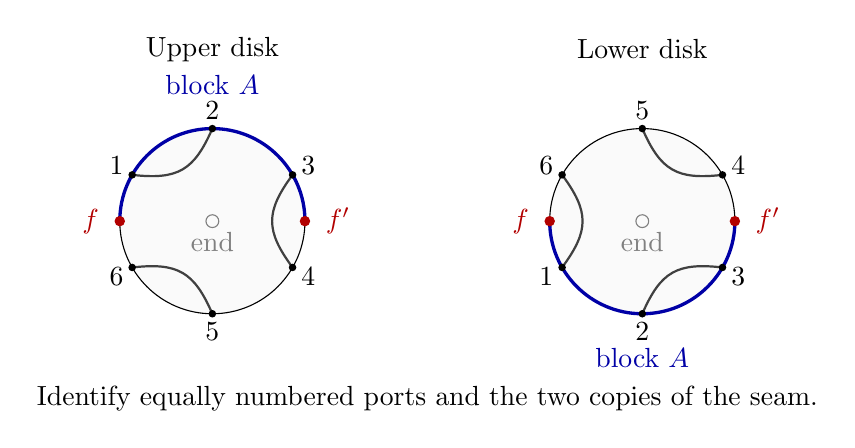
\begin{tikzpicture}[scale=1.05,line cap=round,line join=round,
 arcpath/.style={thick,black!75},seamblock/.style={very thick,blue!65!black}]
\begin{scope}
\draw[fill=gray!4] (0,0) circle (1.12);
\draw[seamblock] (180:1.12) arc (180:0:1.12);
\node[blue!65!black] at (0,1.65) {block $A$};
\node at (0,2.08) {Upper disk};
\draw[arcpath] (150:1.12) .. controls (130:.65) and (110:.65) .. (90:1.12);
\draw[arcpath] (30:1.12) .. controls (10:.65) and (-10:.65) .. (-30:1.12);
\draw[arcpath] (-90:1.12) .. controls (-110:.65) and (-130:.65) .. (-150:1.12);
\foreach \a/\k in {150/1,90/2,30/3,-30/4,-90/5,-150/6}{
 \fill (\a:1.12) circle (1.3pt);\node at (\a:1.34) {$\k$};}
\draw[gray] (0,0) circle (2.2pt);
\node[gray] at (0,-.25) {end};
\fill[red!70!black] (-1.12,0) circle (1.8pt) node[left=4pt] {$f$};
\fill[red!70!black] (1.12,0) circle (1.8pt) node[right=4pt] {$f'$};
\end{scope}
\begin{scope}[xshift=5.2cm]
\draw[fill=gray!4] (0,0) circle (1.12);
\draw[seamblock] (-180:1.12) arc (-180:0:1.12);
\node[blue!65!black] at (0,-1.65) {block $A$};
\node at (0,2.08) {Lower disk};
\draw[arcpath] (-150:1.12) .. controls (-170:.65) and (170:.65) .. (150:1.12);
\draw[arcpath] (-90:1.12) .. controls (-70:.65) and (-50:.65) .. (-30:1.12);
\draw[arcpath] (30:1.12) .. controls (50:.65) and (70:.65) .. (90:1.12);
\foreach \a/\k in {-150/1,-90/2,-30/3,30/4,90/5,150/6}{
 \fill (\a:1.12) circle (1.3pt);\node at (\a:1.34) {$\k$};}
\draw[gray] (0,0) circle (2.2pt);
\node[gray] at (0,-.25) {end};
\fill[red!70!black] (-1.12,0) circle (1.8pt) node[left=4pt] {$f$};
\fill[red!70!black] (1.12,0) circle (1.8pt) node[right=4pt] {$f'$};
\end{scope}
\node at (2.6,-2.14) {Identify equally numbered ports and the two copies of the seam.};
\end{tikzpicture}

\caption{A six-port gluing example. The two disks have opposite boundary
orientations, and equally numbered ports are identified. The hollow
interior marks are the compactified cylinder ends; their faces are
forgotten by the disk state. The seam marks $f,f'$ and the highlighted
block $A$ remain fixed. In the spin pairing this block carries
$m^{\sum_{i\in A}s_i}$, with $m=q^{-2}e^{i\theta}$.}
\label{fig:disk-gluing}
\end{figure}

For an oriented polygon, its arc factors in the two vectors together multiply to \(q^2\) if \(f\) lies to its left, \(q^{-2}\) otherwise (sides can be taken on the sphere compactifying both ends of the cylinder). Indeed flatten that sphere minus \(f\) to the oriented plane with the seam as horizontal line in increasing port order, orthogonality at crossings maintained. For instance in complex plane coordinates of the cylinder use \(\xi=\exp(2\pi i(Z-f)/L)\) with period \(L=2n|U|\), then \(i(1+\xi)/(1-\xi)\). Each upper or lower simple arc has total turn \(-\pi\) times its earlier-endpoint spin, by closing against the line; joins go straight. The polygon turn is \(-2\pi\) if its unbounded side is on its left and \(+2\pi\) otherwise, giving the asserted product of \(q^{s_{\rm earlier}}\). The sum of spins in the initial block for this polygon equals its \(f\)-left indicator minus its \(f'\)-left indicator (the indicator drops across an upward crossing moving positively on the seam). Thus if it separates, the twist \(m\) with the arc product gives \(e^{\pm i\theta}\); otherwise the two orientations cancel since \(q^2+q^{-2}=0\). This proves the interpretation, in particular \(V_{n,n}=1\) at
\(\theta=\pi/2\) and positivity and monotonicity in \(2\cos\theta\ge0\).
Every separator crosses the seam segment from \(f\) to \(f'\) at one
of its \(n\) ports. Disjoint polygons use distinct ports, so there are
at most \(n\) separators. Thus the partition function is a polynomial
in \(2\cos\theta\), with finite nonnegative coefficients. This
physical interpretation is only asserted at balanced homogeneity;
the rapidity-dependent pairing remains an algebraic object.

\paragraph{Scalar reductions.}
We return to generic rapidities. The pairing is separately symmetric by exchange, transpose symmetry of the noncyclic boxes, conservation of total spin there and unitarity. Multiplying by \(p_N(x)^2\) gives polynomial of degrees \(\le2N-2\) each by \eqref{c2:eq-23}, inversion and pairing equal occupancies. Within a block, paired reductions give simple deletion at difference \(3\lambda\) or merging at \(2\lambda\) for \(V\): order adjacently descending in the block. One vector inserts \(L\); the other reduces on application of \(L^t\), since its exchange by \(LL^t\) gives \(L\) of the reduced vector and \(L\) is injective. The twist passes through \(L\) by spin conservation. There is single-site deletion also at zero and infinity, and clustering the adjacent sites on either side of the internal block boundary (say at zero) factors off \(V_{1,1}\).

For clarity, we record these normalized scalar rules explicitly.  Fix
$\theta$ and write $V_{k,l}(X_A;X_B)$, where the subscripts give the lengths
of the two variable lists; put $N=k+l$ and $X=(X_A,X_B)$.  All specializations
below are at generic nonzero values of the remaining variables.  For $k\ge2$,
the two same-block rules in $A$ are
\[
\begin{aligned}
 V_{k,l}(X_A,q^3y,y;X_B)&=V_{k-2,l}(X_A;X_B),\\
 V_{k,l}(X_A,qu,u/q;X_B)&=V_{k-1,l}(X_A,u;X_B).
\end{aligned}
\]
Here $X_A$ has length $k-2$ on both left-hand sides; the identical rules
apply in $B$.  These identities concern the normalized pairing $V$.
After multiplication by $p_N^2$, their scalar factors are the corresponding
factors in \eqref{c2:eq-22}, squared.  For $k\ge1$, single-site deletion is
\[
 \lim_{x\to0}V_{k,l}(X_A,x;X_B)
 =\lim_{x\to\infty}V_{k,l}(X_A,x;X_B)
 =V_{k-1,l}(X_A;X_B),
\]
and likewise in $B$.  For $k,l\ge1$, the two sites adjacent across the
block boundary satisfy, for fixed generic $u,v$,
\[
 \lim_{\varepsilon\to0}
 V_{k,l}(X_A,\varepsilon u;\varepsilon v,X_B)
 =V_{k-1,l-1}(X_A;X_B)V_{1,1}(u;v).
\]
The same $\theta$ is used in all factors.  Separate symmetry permits the
sites involved in a same-block rule to be moved next to each other.

\begin{lemma}[Uniqueness of the scalar pairing]
\label{c2:lem-scalar-uniqueness}
Suppose $V_{k,l}(X_A;X_B)$, for $k,l\ge0$, are separately symmetric
rational functions of the two variable lists.  Assume that
$p_N(X)^2V_{k,l}(X_A;X_B)$ is a polynomial of degree at most $2N-2$ in
each variable for $N\ge1$, and that the deletion, merging, single-site and
two-site scalar rules above hold.  Then the family is determined by
$V_{0,0}$ and $V_{1,1}$.
\end{lemma}

\begin{proof}
Compare two families and choose the least total size \(N\) at which
they differ. Write \(D=p_N^2(V-\widetilde V)\). The single-site rules
make \(D\) vanish at \(x_i=0\) and remove its top coefficient in \(x_i\):
indeed \eqref{c2:eq-22} and inversion give nonzero generic leading and
constant coefficients for \(p_N\). Thus
\(\deg_{x_i}D\le2N-3\). For a site in block \(A\), the pair rules
supply another \(4(k-1)\) distinct generic roots
\(x_i=q^{\pm2}x_j,q^{\pm3}x_j\) with \(j\) in that block.
The corresponding count in block \(B\) is \(4(l-1)\).
If \(k>l\), the first count together with the zero root exceeds
\(2N-3\); if \(l>k\), use the second. Either case forces \(D=0\).
The same single-site argument covers total size one.

When \(k=l\), the roots account for the full degree in every variable.
Hence the only possible difference is a constant times
\[
 \prod_i x_i\ \prod_{i<j\ {\rm same\ block}}
 \prod_{b\in\{2,3,-2,-3\}}(x_j-q^b x_i).
\]
To determine the constant, take one site from each block to zero
proportionally. The two-site rule and minimality of \(N\) give
\(V-\widetilde V=o(1)\); its lower factor and \(V_{1,1}\) agree in
the two families. The two-site limit above shows that \(p_N\) vanishes
linearly along this specialization at generic proportions. Therefore
\(D=o(\varepsilon^2)\). The displayed product vanishes to exactly
order two, so its constant is zero. The prescribed sizes zero and
\((1,1)\) finish the induction.
\end{proof}

\paragraph{An explicit scalar gas.}
The preceding reductions characterize the scalar pairing. We now give
a gas with those reductions and verify all of them. Its labels
\(r_i\in\{-1,0,1\}\) are gas variables, not the spin coordinates
\(s_i\) of the disk vector. Label zero is a vacant gas site; the two
nonzero labels will later become contour residues. The gas sum imposes signed neutrality
\(\sum_A r_i-\sum_B r_i=0\). Its equality with the twisted contraction
will follow from the scalar characterization, rather than a direct
identification of gas labels with spins.

We use a centered version of the fixed scalar polynomial, so that its
pair factors depend on rapidity differences. Put \(\mathfrak p_j(w)=2\sin(w-j\lambda)\) for a rapidity argument; write \(\mathcal P_N=p_N(x)\prod_i x_i^{-(N-1)/2}\) for the centered Pf polynomial. For labels \(r,s=-1,0,1\) in that order use factors \(g_{t,r,s}(w)\), row-column entries with \(t=0\) (same block) or \(1\) (opposite blocks), argument later rapidity minus earlier:
\[
 g_0=
 \begin{pmatrix}
 \mathfrak p_2\mathfrak p_3\mathfrak p_5\mathfrak p_6&-\mathfrak p_3\mathfrak p_5\mathfrak p_6/\mathfrak p_0&\mathfrak p_5\mathfrak p_6/(\mathfrak p_0\mathfrak p_1)\\
 \mathfrak p_2\mathfrak p_3\mathfrak p_5/\mathfrak p_0&\mathfrak p_2\mathfrak p_3\mathfrak p_5\mathfrak p_6/(\mathfrak p_1\mathfrak p_7)&-\mathfrak p_3\mathfrak p_5\mathfrak p_6/\mathfrak p_0\\
 -\mathfrak p_2\mathfrak p_3/(\mathfrak p_0\mathfrak p_7)&\mathfrak p_2\mathfrak p_3\mathfrak p_5/\mathfrak p_0&\mathfrak p_2\mathfrak p_3\mathfrak p_5\mathfrak p_6
 \end{pmatrix},\qquad
 g_1=
 \begin{pmatrix}
 1&\mathfrak p_5^2&\mathfrak p_5^2\mathfrak p_6^2\\
 \mathfrak p_3^2&\mathfrak p_4^2&\mathfrak p_5^2\\
 \mathfrak p_2^2\mathfrak p_3^2&\mathfrak p_3^2&1
 \end{pmatrix}.
\]
\begin{proposition}[Scalar-gas identity]
\label{c2:prop-scalar-gas}
For the two consecutive blocks and the factors just defined,
\begin{equation}
 \mathcal P_N^2 V_{k,l}=
 \sum_{\sum_A r_i=\sum_B r_i=j}
 e^{i\theta j}\mu^{\sum_i |r_i|}
 \prod_{i<h}g_{t(i,h),r_i,r_h}(z_h-z_i),                                \label{c2:eq-24}
\end{equation}
where \(j\) also ranges over the integers.
\end{proposition}

\begin{proof}
We apply Lemma~\ref{c2:lem-scalar-uniqueness}. There are three checks:
cancellation of the apparent poles, agreement with fusion, and the
single-site and two-site limits. We work after dividing the proposed expression by \(\mathcal P_N^2\) at generic parameters. Each matrix has reversal symmetry \(g_t(-w)=g_t(w)^t\), giving the required symmetry of the sum. Thus simple poles at same-block coincidences vanish. At argument \(\lambda\) in that block there are two possible residues, from \((-,+)\) and \((0,0)\); they cancel including the \(\mu^2\) weight (\(\mu^2=2-d\), and \(g_{0,0,0}/g_{0,-,+}=\mathfrak p_2\mathfrak p_3\mathfrak p_0/\mathfrak p_7\) there by cancellation). Spectators see identical factors since
\[
 g_{t,0,v}(u)g_{t,0,v}(u-\lambda)=g_{t,-,v}(u)g_{t,+,v}(u-\lambda).
\]
Use reversal for \(-\lambda\); there are no other finite rapidity poles modulo \(\pi\). With block signs \(\epsilon_i=+1,-1\), the net number of sine powers per pair is \(2+2\epsilon_i\epsilon_h r_i r_h\), even; thus these are rational functions of the \(x\)'s. A term grows at most with power \(N-1-r_i^2\) of \(x_i^{\pm1}\) at infinity and zero by signed neutrality. Multiplying the sum by \(\prod x_i^{N-1}\) now gives a polynomial with the required degrees.

At same-block argument \(2\lambda\) only \((-,0),(-,+),(0,+)\) survive with factors \(2,2+d,2\), and give new label \(r+s\) at the midpoint. At \(3\lambda\) only \((-,+)\) survives with factor one, the pair deleting. In these respective cases
\[
\begin{split}
 g_{t,r,v}(u)g_{t,s,v}(u-2\lambda)&=\mathfrak p_5(u)^2g_{t,r+s,v}(u-\lambda),\\
 g_{t,-,v}(u)g_{t,+,v}(u-3\lambda)&=\mathfrak p_5(u)^2\mathfrak p_6(u)^2 .
\end{split}
\]
All three spectator identities follow by termwise shifts in the displayed arrays, using
\[
 \mathfrak p_j(u-m\lambda)=\mathfrak p_{j+m}(u),\qquad
 \mathfrak p_{j+8}=-\mathfrak p_j.
\] For instance for \((t,r,s)=(0,-,0)\) the quotients by \(g_{t,-,v}(u-\lambda)\) read successively
\[
\begin{gathered}
(\mathfrak p_2\mathfrak p_3\mathfrak p_5\mathfrak p_6)(\mathfrak p_4\mathfrak p_5\mathfrak p_7/\mathfrak p_2)/(\mathfrak p_3\mathfrak p_4\mathfrak p_6\mathfrak p_7) \\
(-\mathfrak p_3\mathfrak p_5\mathfrak p_6/\mathfrak p_0)(\mathfrak p_4\mathfrak p_5\mathfrak p_7\mathfrak p_8/(\mathfrak p_3\mathfrak p_9))/(-\mathfrak p_4\mathfrak p_6\mathfrak p_7/\mathfrak p_1) \\
(\mathfrak p_5\mathfrak p_6/(\mathfrak p_0\mathfrak p_1))(-\mathfrak p_5\mathfrak p_7\mathfrak p_8/\mathfrak p_2)/(\mathfrak p_6\mathfrak p_7/(\mathfrak p_1\mathfrak p_2)) .
\end{gathered}
\]
all \(\mathfrak p_5^2\). Including one-body factors, the new pair constants relative to the lower weights are always \(2\) or \(\mu^2\) in the \(2\lambda\) or \(3\lambda\) case (\((2+d)\mu^2=2\)). Together with the spectator factors these are exactly \eqref{c2:eq-22} squared in centered normalization: for \(z_j=z_i+2\lambda\) the prefactor there before squaring is \(d\prod_{k\ {\rm ext}}2\cos(z_k-z_i-\lambda)\), and for \(3\lambda\) it is \(\mu\prod_{k\ {\rm ext}}\mathfrak p_5(z_k-z_i)\mathfrak p_6(z_k-z_i)\). Each lower label choice has a unique surviving lift.

For the needed clusters (one small variable, one large, or the adjacent cross-block pair small proportionally), place the smaller-in-magnitude group first for the cross products by reversal symmetry. If this group has nonzero signed charge \(a=\sum\epsilon_i r_i\), its relative term decays with scale power \(a^2\) compared to the leading \(\prod_{i\ {\rm small},h\ {\rm large}}x_h/x_i\). Otherwise both groups are neutral and factor independently with leading coefficient one for their interaction. Indeed the constant for large \(x_h/x_i\) in \(g_{t(i,h),r_i,r_h}\) after pulling out \((x_h/x_i)^{1+\epsilon_i\epsilon_h r_i r_h}\) is
\(\exp[i\lambda\epsilon_i\epsilon_h(2-r_i r_h)(r_h-r_i)]\), using \(\mathfrak p_b(w)\sim-i e^{iw-ib\lambda}\). Both phases and extra powers therefore cancel across separately neutral groups by summing exponents. \(\mathcal P_N^2\) has the same product clustering with this leading interaction: use \eqref{c2:eq-22} and inversion for single-variable tests, and the linear term of \(p_N\) above for the pair test. Thus the proposed normalized gas has the required cluster rules (one site alone neutral just contributes one). Size zero is clear and at \((1,1)\) both sides of \eqref{c2:eq-24} equal \(4\cos^2(z_1-z_2)+2\mu^2\cos\theta\). This proves \eqref{c2:eq-24}.
\end{proof}

\subsection{From the scalar gas to contour residues}
\label{c2:sec-contour-representation}

The finite scalar identity has one nonzero label at most at each site.
We encode its occupied sites as residues of contour integrals. The apparent
sum over arbitrarily many contour variables will still be finite: repeated
use of one site has zero residue.
Letters have labels \(X=A,B\) and charges \(R=r e_X,\ r=\pm1\), in a two-dimensional space (unit coordinate vectors). Recall \(\mathfrak p_j(v)=2\sin(v-j\lambda)\),
\[
 K_{AA}=K_{BB}=-\mathfrak p_0^2\mathfrak p_2\mathfrak p_6/(\mathfrak p_1\mathfrak p_7),\qquad K_{AB}=K_{BA}=\mathfrak p_4^2/(\mathfrak p_3^2\mathfrak p_5^2),
 \qquad c_\star=\lim_{s\downarrow0}\sqrt{K_{AA}(is)}/s.
\]
Use the pair factors \(K_{X_iX_j}(v_i-v_j)^{r_i r_j}\), and the one-letter factors \(r c_\star F(v)^{nr}\,dv/(2\pi i)\) with
\[
 F(v)=\frac{\sin(v-\lambda/2)\sin(v+3\lambda/2)\cos^2(v-\lambda/2)}
 {\sin(v+\lambda/2)\sin(v-3\lambda/2)\cos^2(v+\lambda/2)}.
\]
For nonnegative counts \(n_{A,+},n_{A,-},n_{B,+},n_{B,-}\), take the
product of these one-letter and pair factors and divide by
\(\prod_{X,r}n_{X,r}!\). Integrate on small positively oriented circles about \(-r\lambda/2\) and sum over the four counts. Keep \(\sum R_i=(\mathfrak q,\mathfrak q)\), \(\mathfrak q\) unrestricted, and include \(e^{i\theta \mathfrak q}\). Write \(\mathcal Z_n\) for this sum.

\paragraph{Matching the scalar gas with contour residues.}
At balanced homogeneity \eqref{c2:eq-24} is precisely
\[
 p_{2n}(1,\ldots,1)^2 V_{n,n}=(2+d)^{2n(n-1)}4^{n^2}\mathcal Z_n(\theta),
\]
The large factor on the right is the product of all vacant pair
weights. In particular, the physical identity
\(V_{n,n}(\pi/2)=1\) fixes a nontrivial value of
\(\mathcal Z_n(\pi/2)\); it does not normalize that contour gas to one.
To prove the residue identity, abbreviate \(K_0=K_{AA}=K_{BB}\) and \(K_1=K_{AB}=K_{BA}\); the normalization above is \(c_\star=4\cos\lambda\). Extract the product of all \((0,0)\) pair factors from \eqref{c2:eq-24} and associate each nonzero label to a letter at \(v_i=z_i-r_i\lambda/2\). Put \(u_{t,r}=g_{t,0,r}/g_{t,0,0}\). Direct substitution gives, for nonzero charges,
\[
\begin{aligned}
 \frac{g_{t,r,s}(w)g_{t,0,0}(w)}{g_{t,r,0}(w)g_{t,0,s}(w)}
 &=K_t(w-(s-r)\lambda/2)^{rs},\\
 u_{0,r}(w)u_{1,r}(w)&=F(w-r\lambda/2)^r,\\
 r c_\star\operatorname{Res}_{w=0}u_{0,r}(w)&=\mu .
\end{aligned}
\]
For example \(u_{0,+}=-\mathfrak p_1\mathfrak p_7/(\mathfrak p_0\mathfrak p_2),\ u_{1,+}=\mathfrak p_5^2/\mathfrak p_4^2,\ u_{t,-}(w)=u_{t,+}(-w)\); for \((r,s)=(-,+)\) the left quotient is \(\mathfrak p_2\mathfrak p_0/(\mathfrak p_3\mathfrak p_1^2\mathfrak p_7)\) if \(t=0\), \(\mathfrak p_6^2\mathfrak p_4^2/\mathfrak p_5^2\) if \(t=1\), with equal-charge quotients just \(K_t(w)\).

Use identical generic small rapidity lists \((\zeta_j)_{j\le n}\) in each block, replacing \(F(v)^{nr}\) under the integral by \(\prod_j F(v-\zeta_j)^r\). Small circles then enclose simple individual poles at the shifted sites; all pair factors with indicated powers are regular on these small polydisks. Repeating a site within the same block costs a zero (of \(K_0\) at 0 for equal charges, or of \(1/K_0\) at \(\pm\lambda\) for opposite). Thus residues choose nonzero labels on distinct sites in each block, orderings canceled by the factorials. For an active site \(i\), the missing same-block self factor is supplied as \(r_i c_\star\operatorname{Res}u_{0,r_i}=\mu\), while the opposite-block site at the same rapidity contributes the ordinary \(u_{1,r_i}(0)\). The other \(u\) factors and the pair corrections in the identities then give exactly \eqref{c2:eq-24} divided by the extracted product. Take the lists back to zero by continuity (each order with more than \(2n\) letters already vanishes separately); the extracted factor is regular there with same-block value \((2+d)^2\) per pair and cross-block value \(4\).



\section{A contour bound for the two-gap cylinder sum}
\label{c2:sec-contour}

We estimate the homogeneous gas \(\mathcal Z_n\) defined above. Throughout the analysis,
\[
 \nu=\frac{\pi}{3\lambda},\qquad c_s=\frac98,
 \qquad \lambda=\frac\pi8,\quad d=\sqrt2.
\]
\begin{theorem}[Homogeneous gas bound]
\label{c2:thm-contour-bound}
As \(n\to\infty\),
\begin{equation}
 \log|\mathcal Z_n(\theta)e^{-A_\infty n^2}|/\log n
 \ \le\ \tfrac38-\tfrac{2}{3\pi^2}\Re(\theta^2)+o(1),\qquad
 A_\infty=\log\!\big(4(2+d)^2/81\big)                                     \label{c2:eq-V1}
\end{equation}
uniformly in a fixed complex neighborhood of \([0,\pi/2]\).
\end{theorem}

The proof has two analytic steps. In Section~\ref{c2:sec-currents} we
periodize the gas, express it as an oscillator trace, and reflect the
currents. The reflection replaces an oscillating source by a decaying one,
but also replaces the interaction matrix by its inverse. In
Section~\ref{c2:sec-stability} we prove coercivity for this new interaction,
including every residue created when the contours move. These estimates
control the complete sum over particle numbers and permit the period to
return to infinity. The determinant estimate in Section~\ref{c2:sec-normalization} gives sharpness at \(\pi/2\) in the gluing identity
\[
 P_{2n}^2 V_{n,n}(\theta)=(2+d)^{2n(n-1)}4^{n^2}\mathcal Z_n(\theta),
 \qquad P_m=p_m(1,\ldots,1)
\]
(\(p_m\) here is the Pfaffian polynomial, as distinct from the sine factors \(\mathfrak p_j\)). Thus this analysis uses the gluing identity and positivity from the algebra/geometric parts only when applying \eqref{c2:eq-V1}.

\subsection{Elliptic deformation and reflection of currents}
\label{c2:sec-currents}

We begin with a real period \(T\). The period is an analytic device and
will eventually tend to infinity; it is not the circumference of the
physical cylinder. Fourier analysis determines the interaction before we
introduce its oscillator representation.

Take \(T\) large and put \(y=-iv,\ \omega=2\pi/T,\ a=\lambda p\) for Fourier variable \(p\). Use projectors \(P_s,P_d\) onto \((1,1),(1,-1)\), respectively (these projector symbols below do not denote Pfaffians), and write suffixes \(+,-\) for the two corresponding eigenvalues. Set
\[
 M_\pm(p)=\frac{\cosh4a-\cosh3a+\cosh2a\ \pm(1-2\cosh a)}{\sinh4a},
 \qquad M=M_+P_s+M_-P_d .
\]
For \(p>0\) the numerators factor as
\((C-1)(2C-1)(2C+1)^2,\ (C+1)(2C-1)^3,\ C=\cosh a\). At zero \(M_+=c_s a+O(a^3),\ M_-=1/(2a)+O(a)\); at \(+\infty\), \(M=I+O(e^{-a})\).
With physical-axis notation \(\mathcal K_{XY}(s)=\log K_{XY}(is)\) (real there), and transform convention \(e^{-ips}\), we have
\[
 \widehat{\mathcal K-4P_d|\cdot|}=-2\pi\left(M/p-P_d/(2\lambda p^2)\right).
\]
In fact the diagonal and off-diagonal entries of \(\mathcal K\) are \(S_0+S_2-S_1,\ S_4-2S_3\), with \(S_j(s)=\log(4|\sin(is-j\lambda)|^2)\). Expand in \(e^{-2|s|}\): the transform of \(S_j-2|s|\) is \(-8\sum_{h\ge1}\cos(2hj\lambda)/(4h^2+p^2)=-2\pi\cosh((4-j)a)/(p\sinh4a)+4/p^2\), for \(0\le j\le8\). The Fourier sum follows by periodizing a decaying exponential and computing its coefficients.

Replace \(F\) by \(F_T(v)=\prod_{k\in\mathbb Z}F(v+ikT)\) (unit tails); use pair logs
\[
 \mathcal K^T(s)=4P_d|s|+\sum_{k\in\mathbb Z}\left(\mathcal K(s+kT)-4P_d|s+kT|\right),
\]
with the corresponding half diagonal finite part for \(\log c_\star\) (subtract \(2\log|s|\) before taking half), and meromorphic continuation of factors. For coordinates write \(D=\sum y_i R_i,\ Q=\sum R_i\); subscripts \(s,d\) on a vector denote \emph{unnormalized} components (sum, difference). Insert also
\[
 \frac{\sum_{j\in\mathbb Z}\exp(-2Tj^2+4j D_d)}
 {\sum_{j\in\mathbb Z}\exp(-2Tj^2)} .
\]
On the small circles the prescriptions are analytic near nome \(e^{-2T}=0\), with value there the trigonometric integrands (denote the new sum by \(\mathcal Z_{n,T}\)); indeed each nonzero pair image uses the trigonometric ratio divided by its own exponential leading term (continue from bounded real \(s\) with the real sign of the translate), and the self constant uses the branch fixed by \(c_\star\) at nome zero. One can take fixed sufficiently small circles and nome disk independent of \(n\), since the pole positions and this local continuation of the factors do not depend on the powers \(n\). Only orders with at most \(2n\) letters can contribute: split the \(n\) coincident sources into slightly translated ones (same translations for plus and minus on one label). Picking simple residues, repeating a chosen site on that label costs a zero at displacement 0 or \(\pm\lambda\); the other pair factors are regular. Take translations back to zero.

\subsubsection{Oscillator traces and the initial contour deformation}
We represent the elliptic gas as a trace so that a current reflection can exchange the interaction matrix with its inverse. The momentum lattice is
\[
 \mathbf p_A=(\mathbf p_s+\mathbf p_d)/2,\qquad
 \mathbf p_B=(\mathbf p_s-\mathbf p_d)/2,
 \qquad (\mathbf p_s,\mathbf p_d)\in\mathbb Z^2.
\]
Thus the two label momenta are either both integers or both
half-integers. Use the shifts \(V_R|\mathbf p\rangle=|\mathbf p+R\rangle\), and at each level \(m\ge1\) two ordinary oscillators \([a_m,a_m^*]=I\) (on oscillator polynomials: multiplication \(a^*\), derivatives \(a\), orthogonal monomials of norms squared the multifactorials). All independent variables commute. With \(z=e^{\omega v}\) insert fields in smaller-radius-\emph{left} order:
\[
 E_R(v)=\omega V_R z^{-2R\cdot\mathbf p-1}
 \exp\left(-\sum_{m>0}\sqrt{2/m}\,z^{-m}R\cdot a_m^*\right)
 \exp\left(\sum_{m>0}\sqrt{2/m}\,z^m R\cdot a_m\right).
\]
The momentum transfer in \(U\) is \(|\mathbf p\rangle\mapsto w(\mathbf p)|(-\mathbf p_B,-\mathbf p_A)\rangle,\ w=\exp[-\omega\lambda(c_s\mathbf p_s^2+2\mathbf p_d^2)]\). On oscillator monomials it is the induced action of \(r_m=(M-I)(M+I)^{-1}|_{p=m\omega}\). Use \(\operatorname{Tr}(U\,\cdots)/\operatorname{Tr}U\).

To check, the oscillator factor (including \(\omega^N\) for \(N\) letters) on the axis at distinct points has log-modulus
\begin{equation}
 N\log\omega-\sum_{m>0}\frac1m\left(
 \sum_{ij}R_i\cdot M(m\omega) R_j\cos(m\omega(y_i-y_j))-N\right).       \label{c2:eq-V2}
\end{equation}
There are three parts to the trace calculation. First separate the
radii slightly, commute annihilations past creations, and pass to boundary
values. For a scalar oscillator under transfer \(r^k\) on degree \(k\), the normalized trace of \(e^{h a^*}e^{b a}\) equals \(\exp(hb r/(1-r))\) by summing the geometric series and its derivatives. Second, keep the phases and momentum shifts that the log-modulus does
not record. The ordered-commutator phase per \(i<j\) is \(\exp[i R_i\cdot R_j(\omega(y_i-y_j)-\pi\operatorname{sign}(y_i-y_j))]\) on one period by the sine series. The sign product under neutrality is \((-1)^{\mathfrak q^2-N/2}=\prod r_i\). Combining linear parts with all the field powers gives \(\exp[-i\omega D\cdot(2\mathbf p+Q)]\), using initial momentum \(\mathbf p\) on the right. Since the fields first change the rightmost momentum from
\(\mathbf p\) to \(\mathbf p+Q\), the trace closes exactly when
\[
 (\mathbf p_A,\mathbf p_B)
 =(-\mathbf p_B-Q_B,-\mathbf p_A-Q_A).
\]
Equivalently \(Q=(\mathfrak q,\mathfrak q)\) and
\(\mathbf p_s=-\mathfrak q\), while \(\mathbf p_d\) is free.
Gaussian Poisson summation of \(\mathbf p_d\) gives the inserted theta ratio times \(\exp[-\omega D_d^2/(8\lambda)-\omega\lambda c_s \mathfrak q^2]\). Third, compare this answer with the periodized pair and self energies.
The Gaussian factors just obtained supply exactly their zero and
quadratic modes: \(\mathcal K^T-4P_d(s^2/T+T/6)\) on \([-T,T]\) is periodic with modes \(-M(m\omega)/m\) at \(\pm m\), by the transform and the Fourier series of \(|s|-s^2/T-T/6\). The regular mean and the quadratic part, applied to \(Q_d=0\), give the two extra exponents; point-splitting the \(i=j\) singular term gives \(\log\omega\) by the cosine series. This proves the representation using \(F_T(v)^{nr}\eta_X^r E_R(v)\,dv/(2\pi i)\), where \(\eta_A\eta_B=e^{i\theta}\). It also shows the full neutral integrands have imaginary period \(iT\) in each variable.

Take outer axes at \(\pm b\lambda\) in real part of \(v\), for \(b>1/2\) sufficiently close to \(1/2\), and central axes at small \(\pm\epsilon_1\lambda\). Deform the circles coefficientwise to differences of ascending axes: for a plus letter, center (at \(-\epsilon_1\lambda\)) minus left outer axis; for a minus, right outer minus center (at \(+\epsilon_1\lambda\)). Indeed they bound cylinders enclosing the desired respective source poles; no pairwise poles intervene (at relative distance \(\lambda\) between opposite charges one can have zeros). We spell out convergence estimates below. Per label put \(f_X=\eta_X F_T^n\). Let \(C_+\) and \(C_-\) be the ascending central lines at real parts
\(-\epsilon_1\lambda\) and \(+\epsilon_1\lambda\), respectively,
traversed for one imaginary period. For one label define the ordered
contour exponentials by their power series:
\[
 \mathcal E_\pm(g)
 =\exp\!\left(\int_{C_\pm}g(v)E_{\pm e_X}(v)\,\frac{dv}{2\pi i}\right).
\]
At this stage identities are coefficientwise; convergence of the summed
expressions is proved below. The central product can be written
\[
 \mathcal E_+(f_X)\mathcal E_-(-1/f_X)
 =W(f_X)\mathcal E_+(-f_X),\qquad
 W(f)=\mathcal E_+(f)\mathcal E_-(-1/f)\mathcal E_+(f).
\]
Operators on different labels commute in this manipulation.

\subsubsection{The Weyl action and reflected one-body factor}
This is the level-one lattice current construction of
Frenkel--Kac and Segal \cite{FrenkelKac1980,Segal1981}; an explicit
classical realization is given in \cite[Section~2.1]{Frenkel1985}.
The calculation here fixes the action on momentum vacua and the signs
that determine the reflected interaction.

We compute the current reflection on each energy shell, and then its action on the full gas. The energy operator is \(\mathcal H=\mathbf p^2+\sum m a_m^*\cdot a_m\). On one label write \(X_\pm(z)=E_{\pm e_X}/\omega\), and \(e,f_-\) for their integrated zero modes (\(dz/(2\pi i z)\)), without multipliers. They preserve finite-dimensional energy shells, since the \(z\)-power in a field matrix element is energy in minus energy out. On these shells \(e^*=f_-\), by reversing the normal product on the unit circle. Set
\[
 H(z)=2\mathbf p_X-\sum_{m>0}\sqrt{2m}(z^{-m}a_{Xm}^*+z^m a_{Xm}).
\]
Then \([e,X_-(z)]=H(z),\ [f_-,X_+(z)]=-H(z)\); same-sign commutators vanish. In fact the ordered product \(X_+(\zeta)X_-(z)\,d\zeta/\zeta\) after contraction has prefactor \(z(z/\zeta)^{2\mathbf p_X}d\zeta/(z-\zeta)^2\), times the combined oscillator normal product. For the commutator take the negative residue (inner minus outer contour). The calculation is coefficientwise between finite shells, where the radial expansions of the contraction times Laurent polynomials suffice. Also \([H(z),e]=2X_+(z), [H(z),f_-]=-2X_-(z)\) directly by oscillator commutation (the Laurent delta against a field, before taking its zero mode). Thus \([e,f_-]=2\mathbf p_X\), and field coefficients transform in the adjoint representation. Finite-dimensional \(\mathfrak{sl}_2\) on the energy shells gives \(W(1)=\exp(e)\exp(-f_-)\exp(e)\) acting by sign flip on \(H\) (including oscillators) and by \(X_\pm\mapsto-X_\mp\). Its action on a momentum vacuum of this boson sends \(|h\rangle\) to \(\sigma(h)|-h\rangle\); the vacuum field matrix element between \(h,h+1\) gives \(\sigma(h+1)=-\sigma(h)\). Here \(\sigma(0)=1,\ \sigma(-1/2)=1\) from the singlet and defining doublet, respectively (on those minimal-energy vacua the root mode actions are read directly from \(X_\pm\)). Thus the product Weyl sign on the two vacuum labels is
\((-1)^{\mathbf p_d}\). For integer momenta the two signs multiply to
\((-1)^{\mathbf p_A+\mathbf p_B}=(-1)^{\mathbf p_d}\).
For half-integer momenta they multiply to
\((-1)^{\mathbf p_A+\mathbf p_B+1}\), with the same value because
\(\mathbf p_s\) and \(\mathbf p_d\) then have opposite parity.

We now insert the nonconstant source by a Cartan conjugation. Unlike
the zero-mode reflection, this conjugation mixes oscillator levels;
its analytic use will be justified after the contraction calculation.
Define
\[
\begin{gathered}
 \mathcal D=\left(\prod_X\eta_X^{\mathbf p_X}\right)
 \exp\left[-\frac n2\sum_{X,m>0}\sqrt{2m}(L_m a_{Xm}^*+L_{-m} a_{Xm})\right],\\
 L_m=T^{-1}\widehat L(m\omega),\qquad L(y)=\log F(iy).
\end{gathered}
\]
Fixed compatible logarithms can be chosen in the powers. Use the odd imaginary decaying branch \(L\), so that \(\log F_T=L^T\) (periodized) on the axis. Explicitly
\[
 \widehat L(p)=-\frac{2\pi}{p}J(a),\qquad
 J(a)=\frac{\sinh(7a/2)-\sinh(5a/2)-2\sinh(a/2)}{\sinh4a},\qquad L_0=0.
\]
Indeed on \(y>0\), \(L=2i\sum_{h>0}e^{-2hy}[(1+2(-1)^h)\sin(\lambda h)-\sin(3\lambda h)]/h\), with limit zero at 0 by the sine series. In transforming the odd extension, split \(4p/[h(4h^2+p^2)]= (4/p)(1/h-4h/(4h^2+p^2))\); the bracket's \(1/h\) sums cancel, and sum the other terms by differentiating the periodic exponential formula above (or its Abel limit). Cartan commutation now gives \(\mathcal D E_R\mathcal D^{-1}= f_X^r E_R\) near the axis, and hence \(\prod_X W(f_X)=\prod_X W(1)_X\,\mathcal D^{-2}\).

Push this joint \(W(f_X)\) insertion all the way to the left (immediately after \(U\)), converting left outer plus fields times \(f_X\) to minus fields times \(-1/f_X\). The remaining central insertion consists only of plus fields, which can now be taken at 0 in real part, with the two outer axes carrying minus fields. The reflection has three effects on the trace. First, under the new
transfer \(U\prod_X W(1)_X\) the oscillator matrix is \(-r_m\), hence \(M\) is replaced in \eqref{c2:eq-V2} by \(M'=M^{-1}\), with trace ratio \(\prod_{m>0}\det M(m\omega)^{-1}\). Second, the leftmost \(\mathcal D^{-2}\) changes the source and
contributes a common factor \(\exp(n^2 A_T)\), where
\begin{equation}
 A_T=2\sum_{m>0}\frac{m\,L_m L_{-m}}{M_+(m\omega)}.                 \label{c2:eq-V3}
\end{equation}
Indeed its unordered oscillator exponential at level \(m\) has creation and annihilation vectors
\[
 n\sqrt{2m}\,\mathbf 1 L_m,\qquad n\sqrt{2m}\,\mathbf 1 L_{-m},
\]
respectively. Their log self-contraction uses \(M'/2\); against a field on the right they give
\[
 nr[(1/M_+-1)L_m z^m-(1/M_++1)L_{-m}z^{-m}].
\] Thus after including \(F_T^{nr}\) the nonzero modes of the one-body exponent are those of \(nr\log G_T\), with
\[
 G(v)=\frac{\cos(\nu v)-\cos(\pi/6)}{\cos(\nu v)+\cos(\pi/6)},\qquad
 G_T(v)=\prod_{j\in\mathbb Z}G(v+ijT).
\]
In fact
\[
 \frac{J(a)}{M_+(p)}=\frac{\sinh a}{\cosh(3a/2)}.
\]
The same sine-pair transform, now with spacing \(\nu\), gives the transform of \(\log G(iy)\), for \(p>0\), as
\[
 -\frac{2\pi\sinh a}{p\cosh(3a/2)}.
\] Third, the momentum constraint changes. The reflected transfer swaps
rather than negates the two labels, so closing the trace requires
\[
 (\mathbf p_A,\mathbf p_B)
 =(\mathbf p_B+Q_B,\mathbf p_A+Q_A).
\]
Equivalently, \(Q_s=0\) and \(\mathbf p_d=-Q_d/2\), while
\(\mathbf p_s\) ranges over all integers. The constraint \(Q_s=0\)
also cancels the missing common mean in the replacement of the source.
The Weyl vacuum sign, applied after the fields, is
\((-1)^{\mathbf p_d+Q_d}=(-1)^{\mathbf p_d}\), independent of the
remaining momentum sum. Combining the field multipliers with the
\(\eta\)-powers of \(\mathcal D^{-2}\) gives
\(\prod_X\eta_X^{-2\mathbf p_X-Q_X}=e^{-i\theta\mathbf p_s}\).
Since \(2\mathbf p+Q=(\mathbf p_s,\mathbf p_s)\), the linear position
phase is \(e^{-i\omega D_s\mathbf p_s}\). Poisson summation of this
Gaussian momentum sum therefore gives
\begin{equation}
 \Theta_T(\theta,D_s):=
 \sum_{j\in\mathbb Z}
 \exp[-(\theta+2\pi j+\omega D_s)^2/(4\omega\lambda c_s)].
 \label{c2:eq-V4}
\end{equation}

We collect the factors for later use. Put
\[
 \Delta_T=\prod_{m>0}\det M(m\omega)^{-1},\qquad
 \mathcal N_T=
 \frac{\sqrt{\pi/(\omega\lambda c_s)}}
 {\sum_{h\in\mathbb Z}e^{-2\omega\lambda h^2}}.
\]
For a fixed reflected letter list \(\mathcal L\), let
\(\mathcal C_{M'}(\mathcal L)\) denote the right side of
\eqref{c2:eq-V2} with \(M'=M^{-1}\). On distinct physical-axis
positions \(v_i=iy_i\), with \(T>0\) real and \(Q_s=0\), the modulus
of its scalar coefficient before integration and factorials is
\[
 e^{n^2A_T}\Delta_T\mathcal N_T
 \exp\!\left(\mathcal C_{M'}(\mathcal L)
             -2\omega\lambda(Q_d/2)^2\right)
 \prod_i G_T(iy_i)^{nr_i}
 \left|\Theta_T(\theta,D_s)\right|.
\]
Here \(G_T(iy)>0\); the contour and ordering signs have modulus one.
The signed coefficient itself is the trace contraction just computed.
Its extension away from the axis is obtained by meromorphic continuation
of those factors, not by continuation of a modulus.

After collecting the linear phase, the axis logarithms of the signed
pair product are the cosine series in \eqref{c2:eq-V2}. The remaining
ordering signs are constant on each ordered region. High-mode
coefficients expanded in \(x=e^{-a}\) are integral, since \(M\) and
\(M^{-1}\) have integral Taylor coefficients. On any finite-width
strip, extracting finitely many elementary factors associated with
\(\log(1-e^{-\omega k\lambda\pm i\omega s})\) leaves an exponentially
convergent remainder. Thus the continued pair factors have integer
orders of zeros and poles. In Section~\ref{c2:sec-stability} we estimate
this continuation together with the source and momentum factors above.

\subsubsection{Convergence and the operator meaning of reflection}
The algebraic reflection must also hold for the integrated trace. We justify it first for nearby contours, where energy damping gives absolute convergence, and then continue the finite outer-point expressions. Fix a finite list of unintegrated outer points on the two appropriate sides of the center. Initially place them very close to the central axes, all within the Cartan Fourier strip, and take strict radial order very near the unit circle. The old transfer at fixed real \(T\) decays exponentially in energy; indeed \(\|r_m\|\le \exp(-c m\omega\lambda)\) follows by positivity and continuity, with the given small/large-frequency asymptotics. Choose the small central displacements (and the starting positions in this argument) well inside the scale allowed by that decay and by the Cartan coefficients.

\paragraph{Finite products under energy damping.}
Fields between energy shells have the indicated radius powers, and at unit radius \(e^{-\delta\mathcal H}X_\pm e^{-\delta\mathcal H}\) is bounded for every \(\delta>0\). Indeed commute part of the side dampings toward the creation and annihilation coefficients to make them square summable. For square summable vector \(h\), a creation exponential with right-hand damping \(e^{-\epsilon\mathcal H}\) is bounded for each \(\epsilon>0\), and likewise for annihilation (or with damping on the left): on total particle number \(l\), use \(\|(h\cdot a^*)^k\|/\sqrt{k!}\le |h|^k\binom{l+k}{k}^{1/2}\), also bounding annihilations, then the exponential series (\(t^l\binom{l+k}{k}\le(1-t)^{-1-k}\) for \(0<t<1\)). Also \(\operatorname{Tr} e^{-\epsilon\mathcal H}<\infty\) by geometric products. Thus strict radial order and transfers allow absolute multiplication of fixed finite lists on nearby axes by distributing small energy dampings. More explicitly, for radius log \(t\) the bound just given for fields is that
\(e^{(t-\delta)\mathcal H}X_\pm(z)e^{-(t+\delta)\mathcal H}\) is bounded. One puts increasing weights \(u_0< u_1<\cdots<u_k\) across an ordered product in the trace, estimating each insertion \(Y_i\) between \(e^{u_{i-1}\mathcal H}\) and \(e^{-u_i\mathcal H}\) (straddle its radius log for a field). Take the net increase inside the energy decay of the transfer, which preserves shells, so it closes the estimates in trace class. Spare strict gaps and the same trace bound for small dampings make intermediate energy matrix sums absolute.

\paragraph{Cartan conjugations and the central series.}
The same estimates control \(\mathcal D\).
Specifically, \(e^{u\mathcal H}\mathcal D^{\pm1}e^{-(u+\epsilon)\mathcal H}\) is bounded for sufficiently small \(|u|\) and arbitrarily small \(\epsilon>0\): the shifted exponent coefficients decay exponentially and normal ordering followed by the same bounds (inserting a small intermediate loss) uses only small damping loss; momentum factors exponential in the charges do also. In these products one can first cut off the creation/annihilation vectors at finite levels and then pass to limits by the damped estimates, justifying normal-exponential commutations with convergent scalar contractions (in particular the inverse and field conjugations of \(\mathcal D\); for fields take the above two-sided radius margins).

The zero root modes have norms \(O(\sqrt{\mathcal H+1})\) on shells: indeed, writing \(e_h\) for the raising map from charge \(h=\mathbf p_X\), adjointness and \([e,f_-]=2\mathbf p_X\) give \(\|e_h\|^2\le\|e_{h-1}\|^2+2|h|\); iterate using \(|\mathbf p_X|\le\sqrt{\mathcal H}\). These estimates justify Cartan conjugations and integration of powers in the traces there (strictly separate contours slightly where needed; same-sign powers introduce no poles there). In fact at each finite powers product on those contours one can first apply simultaneous Cartan conjugation (cancelling adjacent inverse pairs between the bare fields), then take each bare contour integral as the zero mode. The resulting conjugated products of ordinary zero-root powers can be summed with their factorials with arbitrarily small fixed damping loss, by the shell bound just proved. This applies also to realizing the remaining plus exponential after reflection by contour powers on nearby lines between the strict outer radii. In pushing the insertion, \(W(1)\) preserves shells and acts coefficientwise on each field as above; conjugate by \(\mathcal D\), consuming arbitrarily small parts of the available radius/transfer gaps. This proves the central-exponential identity and the push through finitely many outer fields in that starting neighborhood.

\paragraph{Continuation of the scalar contour evaluations.}
The preceding estimates prove the reflected trace identity with finitely
many outer points in a neighborhood of the central lines. We now use
that identity to reach the outer axes needed for the gas.
Both before and after the push, the contour evaluations of the central exponential series continue with those points to the desired outer radii at generic imaginary coordinates: keep point-to-central distances in real part strictly between 0 and \(\lambda\), avoiding point poles by generic paths/heights; no point-to-central pole intervenes. Absolute convergence of the central evaluations near this continuation, and of the subsequent full outer sums at the chosen radii (so the individual circle deformations and the above identities can be summed and integrated), follows by the real-\(T\) bounds below. This use of continuation avoids asserting an operator trace at remote radii.

\subsubsection{The common scalar factor}
The reflection has isolated the factor \(\exp(n^2A_T)\). To remove the
periodization later, we need its value at infinite period and analyticity
in the small nome. We compute both now.

The quantity \(A_T\) itself extends analytically in the nome \(e^{-2T/3}\) at zero. Put \(l=\omega\lambda\). Then \eqref{c2:eq-V3} is \(-l\sum_{m\in\mathbb Z} H(ml)/(ml)\), where the even function \(H(a)/a\) vanishes at 0 and
\[
 H(a)=J(a)\sinh a/\cosh(3a/2)
 =\frac{x(1-x^2)(1-x)(1-x^3)^2}{(1-x^8)(1+x^3)}
 =\frac{\sum_{j=1}^{23} c_j x^j}{1-x^{24}},\quad x=e^{-a}.
\]
Coefficients \(c_1,\ldots,c_{12}=1,-1,-1,-2,3,3,1,-4,-3,-1,3,2\), with \(c_j=c_{24-j}\) thereafter, follow by multiplication. Poisson summation (periodize the decaying integrand) now has image frequencies \(kT/\lambda\). Shifting Fourier contours past the simple poles \(i\pi j/12\), with bounded residues away from 0, gives a convergent power series in the indicated nome: horizontal contours midway between poles have uniformly exponentially decaying rational factor in real direction. The constant term is
\[
 -2\int_0^\infty H(a)\,\frac{da}{a}=\sum_j c_j\log\sin(\pi j/24)=A_\infty .
\]
Indeed use complete geometric-series packets (\(\sum c_j=\sum j c_j=0\), giving summable integrated packet bounds) and \(\int(e^{-u a}-e^{-v a})\,da/a=\log(v/u)\); pairing reflected indices gives the sine product. We use here the elementary product \(\sin(\pi h)/(\pi h)=\prod_{k\ge1}(1-h^2/k^2)\): for imaginary \(h\) it follows by logarithmic differentiation from the same periodized exponential sum giving \(\sum_{k\in\mathbb Z}1/(k^2+t^2)=\pi\coth(\pi t)/t\), then by analytic continuation. For \(w=\pi/24\), the half-exponent sine product above reduces by double angles to
\(\sin^2(6w)\cos^2w\sin^2(5w)/(2\sin^2(4w)\sin^4(8w)\cos^2(3w))=2(2+\sqrt2)/9\).

\subsection{Stability of the contour expansions}
\label{c2:sec-stability}

The reflection has replaced the interaction by \(M'=M^{-1}\) and the
source by \(G_T\). We must bound the resulting sum uniformly in its
particle order. Two different costs will do this. The long-wave part of
the interaction penalizes the twist \(\theta\), while its remaining
positive energy penalizes particles crowded into a short interval. The
source confines a fixed fraction of the particles to short intervals near
the period ends. Together these estimates give a summable bound.

We first prove the estimates for a real period. They also supply the
absolute convergence used in the preceding current calculation. We then
compare bent contours at complex periods with the real ones and pass to
nome zero. The order of these steps matters: positivity is used only for
the real comparison energy.

\subsubsection{Residue particles and source decay}
Let \(N\) denote the number of elementary letters in one term of the
reflected expansion; it is independent of the source exponent \(n\).
Move the outer minus axes from \(\pm b\lambda\) to
\(\pm\beta\lambda\), where \(\beta=3/2+\kappa\) and \(\kappa>0\)
will be small and fixed. The central plus axis stays at zero.
For either label \(A\) or \(B\), write \(\alpha_t\) for a plus
letter at offset \(t\lambda\); a minus sign reverses its charge.
Residues bind letters at a common longitudinal coordinate. The possible
compound particles are
\begin{equation}
 \gamma_J=\alpha_0-\sum_{t\in J}\alpha_t\quad(J\subset\{-1,1\}),\qquad
 -\alpha_{\pm\beta},\qquad \delta=-\alpha_{-3/2}-\alpha_{3/2}.               \label{c2:eq-V5}
\end{equation}
Here each compound has a single label. The list can be read directly
from the singularities crossed during the two contour moves. In fact the
high-frequency expansion is
\[
 M'=I(1+x)+H_3 x^3+O(x^4),\qquad
 H_3=\begin{pmatrix}-1&2\\2&-1\end{pmatrix}.
\]
Its coefficients at \(x^k\) for \(k\ge1\) are the plus-plus orders at displacement \(\pm k\lambda\), by the log expansions above; order at 0 is \(2I\). The source \(G_T^{-n}\) has no pole between old and new outer radii. Work first at real \(T\). Move left minus fields first: the simple pole at \(-\lambda\) from a center of the same label can bind one such field (a second has cancellation from a double zero). Likewise right minus fields can bind at \(+\lambda\); and they can bind to a free left minus field at distance \(3\lambda\), same label, yielding the across-pair \(\delta\), initially centered at offset \(-\kappa\) and then translated to the indicated symmetric position. 

These moves may be done one point at a time with generic spectators and generic small cut parameters. In the left moves the unbound right minuses are still at \(+b\), too near for the order at distance 3 in offset units; in the right moves any already center-bound left minus is at \(-1\), again too near. A bound left minus does not interfere with right binding at the same center (zero logarithmic order at distance 2).

During the right shifts an already formed across-pair contributes cancellation at a potential aligned binding position by an end-point zero. During translation of across-pairs a minus at an aligned end interacts with nonnegative combined order; two aligned across-pairs give order \(2\) on the same label or \(4\) across labels. They stay at noninteger offsets from center compounds. Two center compounds on the same label have mutual order \(2-|J|-|J'|+2|J\cap J'|\ge0\); the order across labels is zero there. Thus resulting lists have no point-to-point poles on their streams (also for intermediate bound lists in the one-variable moves); the generic residue identities with simple poles integrate directly, with no differentiated factors. 

Here one uses a common representative of the period for the longitudinal points at a binding (in the periodic Poisson sum). At elementary order \(N\) diagram and combinatorial costs are at most \(\exp(O(N\log(N+2)))\), since each unbound-point move branches to at most \(O(N+1)\) terms. Infinite-order convergence is only needed on the pre- and post-deformation sides when summing these coefficient identities.

The functional identities
\[
 G(v-\lambda)G(v+\lambda)=G(v),\qquad
 G(v-3\lambda/2)G(v+3\lambda/2)=1
\]
also determine the source carried by each compound. Write \(G_{T,u}\)
for \(G_T\) evaluated at offset \(u\lambda\), with the same
longitudinal coordinate as the compound. Then
\[
\begin{array}{c|c|c|c}
\text{particle}&\text{elementary letters}&\text{scalar charge}&\text{source}\\ \hline
\gamma_\varnothing&1&1&G_{T,0}^{\,n}\\
\gamma_{\{t\}},\quad t=\pm1&2&0&G_{T,-t}^{\,n}\\
\gamma_{\{-1,1\}}&3&-1&1\\
-\alpha_{\pm\beta}&1&-1&G_{T,\pm\beta}^{-n}\\
\delta&2&-2&1
\end{array}
\]
Call the first two rows \emph{good particles}. If there are \(K\)
compounds, their scalar charges sum to \(Q_s=0\). Each nongood
particle has charge at most \(-1\), whereas a good one has charge at
most \(1\), so at least \(K/2\) are good. Since each compound contains
at most three letters, \(K\ge N/3\); there are therefore at least
\(N/6\) good particles. This is the proportion needed in the final
particle-count estimate.

The scale at which the source confines these particles is
\begin{equation}
 \Re T=B=(2/\nu)\log n,\qquad |\Im T|\le C_{\mathrm{im}}                              \label{c2:eq-V6}
\end{equation}
for sufficiently large fixed \(C_{\mathrm{im}}>3\pi/2\); allowing \(B\) to vary by order one also in continuation. Use streams
\[
 y=s+i(h(s)-u\lambda),\quad -B/2\le s\le B/2,
\]
where \(u\) is the offset and \(h(s+B)=h(s)+\Im T,\ h(\pm B/2)=\pm\Im T/2\). Take \(h=0\) in the period except within a sufficiently large fixed distance of its ends, with arbitrarily small fixed Lipschitz bound, and bounded on the period. The sources of other particles are bounded there by \(\exp(O(1))\) each. Those of good particles are bounded by
\[
 \exp(O(1)-c\,e^{\nu d_s}),\qquad d_s=B/2-|s|,\quad c>0.
\]
Indeed on good offsets the central \(G\) has modulus strictly less than one (\(\Re\cos(\nu v)>0\) on those straight lines) and its real log on the tail is negative of order \(e^{-\nu|s|}\); on outer offsets the modulus is greater than one. Bending near the ends and noncentral images have arbitrary phases but cost bounded error including the power \(n\).

\subsubsection{A coercive quadratic form on the real circle}
Start with a real period \(T=B\). Here is the bound we will prove.
Partition the circle into bins of lengths bounded above and below by
fixed positive constants, and let \(n_l\) count the compounds in bin
\(l\). For a fixed residue list, let \(W_j\) be its integrand with the
source factors and the two common factors
\(\exp(n^2A_T)\) and \(\prod_{m>0}\det M(m\omega)^{-1}\) removed.
It retains the Gaussian normalization, the Poisson branch \(j\), and
the binding and self finite parts. For every fixed \(0<\epsilon<1\),
\begin{equation}
 \sum_{j\in\mathbb Z}|W_j|
 \le C\exp\left\{
 -\frac{(1-\epsilon)B(\theta')^2}{8\pi c_s\lambda}
 -c\sum_l n_l^2+CN\log(B+N+2)\right\}.             \label{c2:eq-real-stability}
\end{equation}
This holds uniformly for real \(\theta'\) in a fixed compact subinterval
of \((-\pi,\pi)\), for all sufficiently large \(B\). The constants may
depend on that interval, \(\epsilon\), and a sufficiently small fixed
\(\kappa>0\). We will keep a positive fraction of the bin-count term
for the later complex-contour comparison. The proof occupies the present
subsubsection and the smearing argument that follows.

We retain two parts of the interaction: a symmetric total-charge pole for the electric cost, and a
strictly positive remainder for the local particle counts. A cross-label
term that is positive only after integration must first be separated
from that remainder.

\paragraph{The real energy and its charge coordinates.}
In the transformed real pair logs with offset difference \(t=|u-v|\le2\beta\) (here \(u,v\) are offset indices) the nonzero Fourier modes are \(-1/m\) times
\[
 \Xi(p;t)=M'(p)\cosh(at)-I\sinh(at)
     -I\sinh(a(t-1)_+)-H_3\sinh(a(t-3)_+),\qquad p=m\omega>0.
\]
Indeed switch each growing elementary log to its decaying expansion: the factor \(\cosh(at)e^{-ak}\) becomes
\[
 \frac{e^{-a(t+k)}+e^{-a|t-k|}}2.
\] At mode zero this crossing adds constant \(\omega\lambda(t-k)_+\) times the expansion coefficient. Thus the real log for branch \(j\) in \eqref{c2:eq-V4} with real twist \(\theta'\), excluding sources and the two common large factors, consists up to harmless normalization of:
\begin{itemize}
\item minus the charge energy with nonzero positive frequencies \(p=m\omega\), kernel \(\Xi(p;t)/m\) on unnormalized Fourier charge sums per offset and label;
\item minus \(\omega/2\) times the regular part at zero of \(\Xi(p;t)/p\) on the row totals (subtract \(P_s/(c_s\lambda p^2)\) first);
\item \(-(\theta'+2\pi j+\omega\sum_i r_i s_i)^2/(4\omega\lambda c_s)\).
\end{itemize}
Indeed \(2\lambda P_d\) in the regular part yields the \(Q_d\) Gaussian; the \(t^2\) part of the leading-pole continuation on \(Q_s=0\) gives exactly the positive log from squaring the imaginary offset sum. Self energies and simple binding-pole energies use point-split finite parts in the additive coordinate.

We specify the charge space on which this energy is coercive. Let
\[
 \mathcal U=\{0,\pm1,\pm3/2,\pm\beta\},\quad
 \mathcal T=\{1,3/2,\beta\},\quad \mathcal O=\{1,\beta\}.
\]
For a particle list, let \(\mu_u^X\) be its signed constituent measure at
offset \(u\lambda\) and label \(X\): a constituent of sign \(r\) at
longitudinal coordinate \(s\) contributes \(r\delta_s\). The central
measures are nonnegative; every noncentral measure is nonpositive.
An across-pair places equal measures at offsets \(3/2\) and \(-3/2\).
Define the unnormalized Fourier sums and their even and odd combinations by
\[
 q_u(p)=\begin{pmatrix}\int e^{ips}\,d\mu_u^A(s)\\
                         \int e^{ips}\,d\mu_u^B(s)\end{pmatrix},\qquad
 q_t^{\rm e}=q_t+q_{-t},\quad q_t^{\rm o}=q_t-q_{-t}.
\]
Thus \(q_{3/2}^{\rm o}=0\). The independent coordinates are
\[
 \mathbf z=(q_0,q_1^{\rm e},q_{3/2}^{\rm e},q_\beta^{\rm e},
                   q_1^{\rm o},q_\beta^{\rm o})\in(\mathbb C^2)^6.
\]
At frequency \(p>0\), their quadratic form is
\begin{align*}
 \mathscr Q_p(\mathbf z)
 &=q_0^*M'q_0+2\Re\sum_{t\in\mathcal T}q_0^*\Xi(p;t)q_t^{\rm e}\\
 &\quad+\sum_{t,u\in\mathcal T}
 (q_t^{\rm e})^*\frac{\Xi(p;|t-u|)+\Xi(p;t+u)}2q_u^{\rm e}\\
 &\quad+\sum_{t,u\in\mathcal O}
 (q_t^{\rm o})^*\frac{\Xi(p;|t-u|)-\Xi(p;t+u)}2q_u^{\rm o}.
\end{align*}
These factors of two follow from using sums and differences, without
normalizing the even and odd coordinates.

\paragraph{A cross-label interaction positive after integration.}
Complete squares in the even part using \(\Xi(p;0)=M'\). We single out
the cross-label entries of the remaining matrix because their inverse
Fourier transforms have a sign on the measures at hand. Put
\(P_t=\sinh(at)+\sinh(a(t-1)_+)\). The remaining Schur entries are
\[
 I\,[\cosh(at)P_u+\cosh(au)P_t-(P_{|t-u|}+P_{t+u})/2]
 -M P_tP_u-H_3\sinh(a(t+u-3)_+)/2 .
\]
Subtract just their cross-label part, whose \(AB\) entry is
\[
 E(a;t,u)=\frac{(2\cosh a-1)P_tP_u}{\sinh4a}-\sinh(a(t+u-3)_+).
\]
In terms of the specified coordinates, the removed form is
\[
 \mathscr E_p(\mathbf z)=\sum_{t,u\in\mathcal T}E(a;t,u)
 \big(\overline{(q_t^{\rm e})_A}(q_u^{\rm e})_B
       +\overline{(q_t^{\rm e})_B}(q_u^{\rm e})_A\big).
\]
It has nonnegative \emph{integrated} energy: \(E/p\) has nonnegative
inverse Fourier transform, and the even charges on noncentral rows are
nonpositive measures. This assertion concerns the Fourier sum, including
the regular zero mode; it does not assert that \(\mathscr E_p\) is
nonnegative at each frequency. To see the transform, sum over \(i=t,t-1,\ j=u,u-1\). Each term uses one half of the difference at \(b=i+j,i-j\) of
\[
 [\cosh(a(b+1))+\cosh(a(b-1))-\cosh(ab)]/(p\sinh4a),
\]
folding \(b+1\) to \(7-b\) when \(b>3\) (this gives the subtracted \(\sinh\)). By the transform for \(S_j\) (with general real \(0\le j\le8\)), the inverse of each folded difference, up to positive factor, is
\[
 \log\frac{J_y(d_0)}{J_y(c_0)},\quad
 J_y(c)=\frac{y^2+\sqrt2 yc+c^2-1/2}{y+c},\quad
 c_0=\cos(\pi(i+j)/4),\quad d_0=\cos(\pi(i-j)/4),
\]
with \(y=\cosh(2s)\). This integrable kernel includes the regular zero mode (periodize for the frequency sum). It is nonnegative: \(d_0\ge c_0,\ c_0+d_0\ge0,\ c_0\ge-0.8\) for small \(\kappa\), hence \((\sqrt2-1)y^2+y(c_0+d_0)+c_0d_0+1/2>0\), which gives the log order (by limits at singularities). Indeed the sign of \(J_y(d_0)-J_y(c_0)\) follows by multiplying this positive expression by \(d_0-c_0\) and dividing by \((y+c_0)(y+d_0)\). Thus on smooth smeared rows (used below) the full energy of the subtracted term is nonnegative by Fourier pairing: the \(1/m\) nonzero-frequency weight and regular zero term together give \(\omega/2\) times the sum over all integer modes with kernel \(E/p\), including its limit.

\paragraph{Strict positivity of the remaining frequency form.}
After the preceding term is removed, the complementary form satisfies
the pointwise estimate
\[
 \widetilde{\mathscr Q}_p(\mathbf z)
 :=\mathscr Q_p(\mathbf z)-\mathscr E_p(\mathbf z)
 \ge c_\kappa\min(a,1)\|\mathbf z\|^2,\qquad p>0.
\]
Here \(\kappa>0\) is fixed and sufficiently small; the constant may depend
on this contour separation. We give the algebraic and perturbation details. In the odd block first take \(\beta=3/2\) in the two matrices on distances \(1,\beta\) (one per \(\pm\) channel), and put \(\zeta=e^{a/2}\). Their first diagonals factor as
\[
 \frac{(\zeta^4-1)(2\zeta^8\pm2\zeta^6+3\zeta^4\pm2\zeta^2+2)}{4D_\pm},
 \quad D_+=(\zeta^4+\zeta^2+1)^2(\zeta^4-\zeta^2+1),\quad
 D_-=(\zeta^4-\zeta^2+1)^3;
\]
their determinants are \((\zeta^2-1)^2/(16D_\pm)\) times respectively
\(2\zeta^8+4\zeta^6+7\zeta^4+4\zeta^2+2,\ 10\zeta^8-16\zeta^6+23\zeta^4-16\zeta^2+10\), positive on \(\zeta\ge1\) (for the latter divide by \(\zeta^4\) and use \(\zeta^2+\zeta^{-2}\ge2\)). The even Schur same-label submatrix on \(1,3/2\) has first diagonal \((\zeta^4-1)(\zeta^4-\zeta^2+1)/(4(\zeta^8+1))\), determinant \((\zeta^2-1)^2(\zeta^4+1)/(16(\zeta^8+1))\). These identities result by substituting \(\sinh(ak),\cosh(ak)=(\zeta^{2k}\mp\zeta^{-2k})/2\), respectively, into the difference kernel and Schur entries above. Entries are \(O(\min(a,1))\) (the common leading pole cancels). Thus these base matrices have the required strict bounds.


\emph{Bounded frequencies and separation of the new row.}
On bounded \(a\)-intervals down to 0 the odd bound persists for small \(\kappa\) by one-sided smooth perturbation (changes \(O(a\kappa)\)). For the even Schur part the new distance \(\beta\), taken in difference from \(3/2\), adds a diagonal \(a\kappa+O(a\kappa^2)\) with couplings \(O(a\kappa)\) to the old. Indeed in the same-label entries the only nonsmooth contribution to the diagonal second difference to first order comes from \(-P_{|t-u|}/2\); all \(t+u\) near 3 here are on the same side. This proves strict bounds on these ranges.

\emph{Large frequencies.}
Uniformly for large \(a\) the folded expansion is
\[
 \Xi(t)=I e^{-at}+\tfrac12 I(e^{-a|t-1|}+e^{-a(t+1)})
 +\tfrac12 H_3(e^{-a|t-3|}+e^{-a(t+3)})+O(e^{-c a})
\]
at the used separations, with the vanishing terms/remainders having one-sided derivative \(O(a e^{-c a})\) where away from their singular offsets. Thus the odd block has negligible off-diagonals and diagonals with leading eigenvalues at least \(1/4\). The even same-label Schur block has leading \(1/4\) at distance 1 with negligible off-block coupling, and on \(3/2,\beta\) the leading matrix
\[
 \tfrac14\begin{pmatrix}1&j\\ j&2-j^2\end{pmatrix},\qquad j=e^{-a\kappa}.
\]
Errors are \(O(e^{-c a})\) and on their difference row/column have an additional factor \(\min(a\kappa,1)\) by the derivative bound. Using sum and difference, the leading matrix controls the sum square and \(\min(a\kappa,1)\) times the difference square. Thus the large-\(a\) threshold can be fixed uniformly before taking small fixed \(\kappa>0\). 

Square completion used bounded column operations (\(M\Xi(t)\) bounded from the folded formula and zero asymptotics), and \(M'\) itself has the lower bound. Together these estimates prove the stated bound. 

At frequency zero the
coordinates are real row totals, and the constraint is exactly
\[
 Q_s=\mathbf1^t\left(q_0+\sum_{t\in\mathcal T}q_t^{\rm e}\right)=0,
 \qquad \mathbf1=(1,1)^t.
\]
The common pole of \(\mathscr Q_p\) is
\(\|P_s(q_0+\sum_tq_t^{\rm e})\|^2/(c_s\lambda p)\), which vanishes
on this subspace. Consequently its modified regular zero form obeys
\[
 \lim_{p\downarrow0}\frac{\widetilde{\mathscr Q}_p(\mathbf z)}p
 \ge\lambda c_\kappa\|\mathbf z\|^2.
\]
This limit enters the energy with coefficient \(\omega/2\); the
positive-frequency forms enter with coefficient \(1/m\).

\paragraph{Retaining the long-wave electric energy.}
For any fixed \(0<\epsilon<1\) we can still keep such a positive bound after subtracting from the \emph{symmetric-channel total} the additional common kernel
\[
 (1-\epsilon)|\widehat h_R(p)|^2/(c_s a),
\]
multiplying the squared norm of \(P_s\) applied to the sum of all charge rows, where \(h_R\) is a smooth nonnegative even compactly supported mass-one mollifier of sufficiently large fixed scale \(R\). For small \(a\) (before choosing \(R\)), even keeping \(\epsilon\) fraction of the leading total pole suffices since on its null subspace the positive bound above applies unchanged, and cross couplings to it are only \(O(a)\). For larger \(a\) choose \(R\) by Fourier decay.

\paragraph{The initial contours.}
The preceding estimates concern the residue contours. The current
reflection also used absolute convergence on its initial contours.
For the real-\(T\) contour manipulations on those lines, a similar positive bound holds without the cross-label subtraction or the extra pole extraction. For \(M'\) use lines \(0,\pm b\); for \(M\) use \(\pm\epsilon_1,\pm b\) in offset units, with the same folding convention using its own high-frequency coefficients. The original leading pole is \(P_d/(2a)\), with total-zero constraint \(Q_d=0\); the original Poisson Gaussian and charge weight reconstruct the regular zero form analogously. To check positivity, start on \(0,\pm1/2\). In each channel with central entry \(D=M_\pm\) or \(M_\pm^{-1}\), the odd entry and remaining even Schur entry are
\(\sinh(a)(1-D\tanh(a/2))/2,\ \sinh(a)(1-\tanh(a/2)/D)/2\). Both have the strict bound by the factorizations of \(M_\pm\): \(M_+>\tanh(a/2),\ M_-<\coth(a/2),\ M_-\ge M_+\), where comparing numerators after cancellation gives \(4C^2+2C-1>0,\ -12C^2+10C-1<0\) for the first two tests, so margins in the entries are nonvanishing multiples of \(\min(a,1)\). Square-completion coefficients again are bounded. Perturb first to \(b>1/2\), with \(O(a|b-1/2|)\) changes on compact intervals (one-sided folding). When needed split the center into \(\pm\epsilon_1\): the even sector has unchanged leading pole and \(O(a\epsilon_1)\) error there, the new odd diagonal is \(a\epsilon_1+O(a\epsilon_1^2)\) from the distance cusp, with couplings \(O(a\epsilon_1)\). At large \(a\) the only nonnegligible off-diagonals in original row coordinates are between the two outer lines (coupling at most \(1/2+o(1)\) by the order-1 term \(\pm I e^{-a}\) before folding) and between the split central lines (leading \(I e^{-2a\epsilon_1}\) with unit leading diagonals). Differences of errors for the central rows have the factor \(\min(a\epsilon_1,1)\) by the same one-sided derivative estimate, giving the bound as above. Choose the position parameters sufficiently small accordingly.

\subsubsection{Smearing, the electric cost, and particle-count bounds}
We now convert the quadratic-form estimate into a bound on the actual
integrand. The comparison is one-sided: after collecting each pair of
compound particles, its point interaction is bounded above by the
interaction of suitably smeared charges, with a controlled loss at
internal finite parts. Work first on the real circle. Replace elementary point rows by smeared measures in the \(s\)-variable using the circular Poisson kernel \(\mathcal P_\rho\) of width \(\rho=(B+N+2)^{-4}\) (convolution multiplier \(e^{-|m|\omega\rho}\), positive density proportional to \((1-2e^{-\omega\rho}\cos(\omega s)+e^{-2\omega\rho})^{-1}\), mass one). We compare the original finite parts with the smeared energy. The total
error is \(O(N\log(B+N+2))\), uniformly in particle order. The estimate
must be applied to whole compound particles: elementary pairs can have
negative logarithmic coefficients before their residues are combined.


Here are the quantitative details of the smearing comparison.  Fix the
contour separation $\kappa>0$.  For every used offset difference $t$,
put $C_t=\lim_{p\to\infty}\Xi(p;t)$.  The pole at zero and the folded
exponential expansion imply, with constants allowed to depend on
$\kappa$,
\[
 \|\Xi(p;t)-C_t\|\le
 \begin{cases}C/p,&0<p\le1,\\ Ce^{-cp},&p\ge1.\end{cases}
\]
Indeed the only terms of the folded expansion that do not decay are
those whose shifted distance is zero; these are precisely $C_t$.
The finite set of other distances has a positive minimum after
$\kappa$ is fixed.  For $B\ge2$, $\omega=2\pi/B$, the smooth remainder
of each pair kernel is
\[
 R_{B,t}(s)=-2\sum_{m\ge1}
          \frac{\Xi(m\omega;t)-C_t}{m}\cos(m\omega s),
 \qquad \|R_{B,t}'\|_\infty\le C(1+\log B).
\]
The last estimate follows by splitting the differentiated series at
$m\omega=1$: the first part is bounded by a harmonic sum and the
second by a geometric sum.

The circular Poisson kernel $\mathcal P_\rho$ is a probability density
and satisfies $\mathcal P_\rho*\mathcal P_\rho=\mathcal P_{2\rho}$.
Writing $|s|_B$ for circular distance to zero, for $0<\rho\le1$ we have
\[
 \int |s|_B\mathcal P_{2\rho}(s)\,ds
       \le C\rho\bigl(1+\log(B/\rho)\bigr).
\]
Consequently replacing a smooth pair remainder by its twice-smeared
version changes it by at most
\[
 C\rho\bigl(1+\log(B/\rho)\bigr)(1+\log B).
\]

For the singular part put $L_B(s)=\log|1-e^{i\omega s}|$.  Its exact
Poisson average and a one-sided comparison are
\[
 (\mathcal P_{2\rho}*L_B)(s)
   =\log|1-e^{-2\omega\rho+i\omega s}|,
 \qquad L_B(s)\le(\mathcal P_{2\rho}*L_B)(s)+\omega\rho.
\]
For the inequality, square both sides after exponentiation and use
$e^{2\omega\rho}+e^{-2\omega\rho}\ge2$.
Apply this inequality after collecting all elementary interactions
between a pair of compound particles.  Their total coincident-log
coefficient is nonnegative; individual elementary interactions need
not have this property.  All constituents of one compound have the
same longitudinal coordinate, so the collection uses one and the
same $L_B(s-s')$.

For a diagonal or binding finite part, subtraction is in the additive
coordinate: $L_B(s)-\log|s|\to\log\omega$ as $s\to0$.  In contrast,
the smeared singular part at zero is
$\log(1-e^{-2\omega\rho})=\log\omega+\log(2\rho)+O(\omega\rho)$.
Their difference is therefore $O(1+|\log\rho|)$, with the
$\log\omega$ terms cancelling.  There are $O(N)$ such internal terms
and $O(N^2)$ external pairs, with uniformly bounded constituent
multiplicities and log coefficients.  On taking
$\rho=(B+N+2)^{-4}$, the total comparison error is
\[
 O\!\left(N(1+|\log\rho|)
   +N^2\omega\rho
   +N^2\rho(1+\log(B/\rho))(1+\log B)\right)
 =O\bigl(N\log(B+N+2)\bigr).
\]
This compares finite parts as well as the off-diagonal kernel and
preserves the nonpositive signs of all noncentral even-row measures.
The same comparison applies at fixed real \(T\) on the initial lines:
independent same-sign letters have nonnegative coincident orders, and the
other line separations are nonsingular.

\paragraph{The electric cost.}
For the smeared energy the nonnegative off-label Schur term can now be
dropped, and the long-wave pole can be retained, as proved above. The extracted pole and \(1-\epsilon\) fraction of the Gaussian give log contribution at most
\[
 -\frac{(1-\epsilon)B}{8\pi c_s\lambda}\,
 \mathop{\rm avg}\big|\theta'+2\pi j-2\pi(h_R*\mathcal P_\rho*H_0)(s)\big|^2 ,
\]
where \(H_0\) is periodic integer cumulative sum of scalar charges \(r_i\) from just before the representative period, with mean \(-\sum_i r_i s_i/B\). This is Parseval (nonzero coefficients of \(H_0\) are the unnormalized Fourier charges divided by \(2\pi i m\)); zero-frequency regular estimates are unchanged under the null-total constraint. Outside length \(O_R(N)\) around jumps the convolved height is within \(O(N\rho)\) of an integer. Thus for \(|\theta'|<\pi\) the suppression cost in log is at least \((1-\epsilon)B(\theta')^2/(8\pi c_s\lambda)-O(1+N)\), with a spare bound of order \(Bj^2\) for \(|j|\) larger than a sufficiently large multiple of \(N+1\) (then the convolved height is itself uniformly bounded by \(N\)).

\paragraph{Local particle counts and the convergence needed earlier.}
Use the bin counts \(n_l\) specified in
\eqref{c2:eq-real-stability}. The remaining coercive energy bounds
\(c\sum_l n_l^2\). In fact its Fourier prefactors on unnormalized smeared row sums are at least \(c/[B(1+p)]\) and at zero at least \(c/B\) under the constraint. Thus by Parseval they control integrated squares of further convolution with a periodized fixed nonnegative smooth bump positive on bin-size neighborhoods (its line transform decays rapidly; take compact support). Each elementary charge contributes density bounded below in magnitude throughout its bin after the two convolutions. Since charges on each used offset/label have fixed sign, this controls the asserted bin counts. Together with the finite-part loss and the electric estimate, this
proves \eqref{c2:eq-real-stability}; the spare large-\(j\) Gaussian
bound sums the remaining Poisson branches.

For fixed real \(T,n\) the initial contours have only \(O_T(1)\)
bins. Their positivity estimate therefore gives, by Cauchy--Schwarz,
\[
 \sum_l n_l^2\ge c_T N^2,
 \qquad
 \exp\big[-c_TN^2+O_{T,n}(N\log(N+2))\big]
\]
as a bound on either the original or the reflected expansion, including
its combinatorial costs. This is summable in \(N\); no source refinement
is needed for this fixed-period assertion. Shifted real Gaussian sums cost bounded factors after accounting for imaginary-offset additions included in the regular zero form (complex twist gives at most \(\exp(O_T(1+N))\) besides). For the central operator step with fixed finite generic outer points only use the bound on the central subspace; finite point couplings there cost \(O_{T}(N)\) locally in the continuation, and any failure of the central totals \emph{alone} to satisfy the zero constraint is a fixed charge so the regular zero comparison has at most linear extra errors. These fixed-period estimates justify the earlier absolute-convergence
claims.

\subsubsection{Continuation to complex periods}
The real estimates have now justified the initial contour sums and the
current reflection. To obtain the bound at nome zero, we need them also
for bounded imaginary parts of the period in \eqref{c2:eq-V6}. We compare
with the real energy; no positive quadratic form is asserted on the bent
contours.

\paragraph{A kernel suitable for continuation.}
Inverse-transform
\[
 \widehat g(p)=-2\pi\left(M'(p)/p-P_s/(c_s\lambda p^2)\right),\qquad
 L_*=\pi P_s/(c_s\lambda),\qquad k(s)=L_*|s|+g(s).
\]
As in the pre-reflection computation, use \(k^T(s)=L_*|s|+\sum_j g(s+jT)\) on real coordinates first (representative point differences in \((-T,T)\)); subtract \(L_*(s^2/T+T/6)\) for its periodic Fourier form. Inserting this kernel (with finite parts as above) now absorbs the mode and charge factors and the \(D_s^2\) part of the Poisson exponent: the quadratic contribution is \(-\pi D_s^2/(2c_s\lambda T)\) by \(Q_s=0\), the regular mean gives \(-\omega\lambda Q_d^2/2\). Thus use continuation of \(k^T\), leaving the external exponent at index \(j\)
\begin{equation}
 -\frac{T(\theta+2\pi j)^2}{8\pi c_s\lambda}
 -\frac{(\theta+2\pi j)D_s}{2 c_s\lambda}.                              \label{c2:eq-V7}
\end{equation}
(In pair logs branches can be taken by continuation sidewise; fixed phase signs have no effect.)

Here are useful regularity details. The even transform defining \(g\) is regular at zero, conditionally invertible off \(s=0\), with poles on the imaginary lattice \(i\nu\mathbb Z\setminus\{0\}\), of bounded order and bounded principal coefficients by the displayed rational factorizations. For real \(s>0\) shift Fourier contours up successively halfway between poles. Horizontal integrals of the \(O(1/|p|)\) tail are bounded before the shift damping, by integration by parts at fixed \(s>0\) (first derivatives integrable uniformly on those lines). Thus residues expand \(g\) in decaying exponentials with polynomial prefactors of bounded degrees/coefficients. This gives continuation on \(\Re s>0\) with exponential decay, also for its derivative when \(\Re s\to+\infty,\ |\Im s|=O(1+|\Re s|)\); similarly on the left. Near bounded separations
\[
 k(s)-I\log(s^2)-I\log(s^2+\lambda^2)-H_3\log(s^2+9\lambda^2)
\]
extends analytically to \(|\Im s|<4\lambda\). Indeed its second derivative has exponentially integrable transform there: the linear absolute term cancels the subtracted zero pole after differentiation, and each \(\log(s^2+b^2)\) has second-derivative transform \(2\pi |p| e^{-b|p|}\). The latter follows by differentiation of the elementary Cauchy kernel transform, with the \(b=0\) limit as distributions. Now use the high-mode expansion; integrating the regular derivative proves the assertion up to harmless affine terms. This also justifies the transforms with real log singularities.

\paragraph{Comparison with the real contours.}
Compare complex positions to their straight counterparts at real \(B\),
with real comparison twist \(\theta'=\Re\theta\). For each real signed longitudinal difference \(x\), including period translates, the imaginary longitudinal change due to bending/period is at most \(\|h'\|_\infty |x|\). The real part of the unsummed signed linear term (continue with the given real sign) is unchanged. Each image remainder therefore costs \(O(\|h'\|_\infty(1+|x|)e^{-c|x|})\): far away by the derivative decay, and nearby by the local logs and strip analyticity (choose the slope sufficiently small). Even at a shifted log singularity, changing imaginary difference by this much only changes the real log by \(O(\|h'\|_\infty)\) at approach; the same bound applies to binding/self finite parts. Summing by bins gives at most \(C\|h'\|_\infty\sum_l n_l^2\), absorbed by the spare coercivity. 

The change of real part in \eqref{c2:eq-V7} is \(B(\Im\theta)^2/(8\pi c_s\lambda)+O(N+1+|j|)\) exactly up to that error (the imaginary part of \(D_s\) stays \(O(N)\)). Normalizing Gaussian factors other than those treated explicitly stay bounded, by the same convergent Gaussian sums/Poisson formula. Sum indices \(j\) with the spare large-\(j\) bound.

\paragraph{Summing all particle orders.}
Combining \eqref{c2:eq-real-stability} with the complex-contour
comparison and the source bound, extract the common factors and the
electric estimate. The total logarithmic absolute cost at elementary order \(N\), including diagram
counts and integration measures, is bounded up to \(O(1)\) by the
supremum of
\[
 C N\log(B+N+2)-c\sum_l n_l^2-c\sum_{\rm good} e^{\nu d_s}.
\]
To see the suppression, put \(L_N=2\log(N+2)/\nu\). If at least
half of the good particles satisfy \(d_s\ge L_N\), their source cost
alone is at least \(cN(N+2)^2\). Otherwise at least \(N/12\)
particles lie in the two end regions \(d_s<L_N\), which together meet
\(O(\log(N+2))\) bins. Cauchy--Schwarz then gives
\[
 \sum_l n_l^2\ge c\frac{N^2}{\log(N+2)}.
\]
In either case the two negative terms dominate
\(c'N^2/\log(N+2)\). For \(N\le(\log B)^3\) the positive term is
\(O((\log B)^4)=o(B)\). Above that threshold it is absorbed by half
of this suppression, uniformly for large \(B\), and the remaining tail
is summable. Thus the complete particle sum costs only \(\exp(o(B))\).

\paragraph{Holomorphic dependence and the continued identity.}
These estimates also justify continuation of the identity, not only an
absolute bound on formal integrands. For fixed large \(n\), put \(B_n=(2/\nu)\log n\) and parametrize streams by \(y=s+(T-B_n)\chi(s)-iu\lambda\), \(\chi(\pm B_n/2)=\pm1/2\), supported near the ends, real with small derivative and period-lifted by 1. On an open rectangle near those periods reparametrize by actual real coordinate for the uniform bounds just proved. The parametrized lists are holomorphic there. To see this, remove sufficiently many of the elementary log factors from the high-mode series as above (depending on the bounded complex period range), leaving locally exponentially summable tails. \par
The possible collisions require a point difference equal to an integer
offset modulo the period. Equality of the real longitudinal parts modulo the period forces the bent heights also to agree modulo its lift, so there are the very same nonnegative interparticle alignment orders, and no new poles (at real longitudinal zero for sources the lift is zero). Indeed the coinciding orders between compounds use the very same longitudinal difference (all offset constituents move together), so cancel meromorphically. Internal simple-binding residues are just regular parts times the other inserted factors. \par
Thus the parameter integrals are holomorphic, and their full sum
converges locally uniformly by the bound just proved. At real \(T\) therein the identity held by the coefficientwise moves and summability on both sides, so it continues to the rectangle.

\subsubsection{The oscillator determinant and the nome limit}
The oscillator determinant is
\[
 \det M=\frac{(1+x^3)^4(1-x^3)^2}{(1+x)^2(1-x^8)^2}.
\]
Integrating its logarithmic series gives
\[
\begin{split}
 -\int_0^\infty\log\det M\,da
 &=-4\frac{\pi^2}{36}+2\frac{\pi^2}{18}
    +2\frac{\pi^2}{12}-2\frac{\pi^2}{48}\\
 &=\frac{\pi^2}{8}.
\end{split}
\]
Here we used
\(\int_0^\infty\log(1-e^{-ka})\,da=-\pi^2/(6k)\) and
\(\int_0^\infty\log(1+e^{-ka})\,da=\pi^2/(12k)\). Riemann summation, uniform also with the bounded imaginary period parts, gives log-modulus of \(\prod_{m>0}\det M(m\omega)^{-1}\) equal to \(B\pi^2/(8\cdot2\pi\lambda)+o(B)\). Since \(B=(2/\nu)\log n\), the determinant contributes
\(\pi/(8\lambda\nu)=3/8\) on the logarithmic scale. The electric
coefficient is \(1/(4\pi c_s\lambda\nu)=2/(3\pi^2)\).
Together with the particle bound, these give the log-modulus divided by
\(\log n\), after removing \(\exp(A_T n^2)\), at most
\[
 \frac38-\frac{2}{3\pi^2}\big((1-\epsilon)(\Re\theta)^2-(\Im\theta)^2\big)+o(1)
\]
on \eqref{c2:eq-V6}, uniformly for bounded complex \(\theta\) near the real segment. The analytic factor \(A_T\) from \eqref{c2:eq-V3} agrees by continuation with its nome series there. Put \(q_T=e^{-2T/3}\). At fixed \(\Re T=B\), an interval of
imaginary parts of length \(3\pi\) traverses the entire circle
\(|q_T|=e^{-2B/3}\); our choice \(C_{\mathrm{im}}>3\pi/2\)
therefore supplies its maximum. The initial small-circle prescription is
holomorphic at \(e^{-2T}=q_T^3=0\), and \(A_T\) is holomorphic in
\(q_T\). The maximum principle applied to
\(\mathcal Z_{n,T}\exp(-A_Tn^2)\) gives the same upper bound at
\(q_T=0\), where it equals
\(\mathcal Z_n\exp(-A_\infty n^2)\). For each fixed
\(\epsilon>0\) the error tends to zero uniformly on the stated compact
angle sets. Take the upper limit as \(n\to\infty\), then let
\(\epsilon\downarrow0\). This proves \eqref{c2:eq-V1}.

\section{Determinant normalization and saturation}
\label{c2:sec-normalization}

The contour estimate bounds a normalized scalar gas. To recover the
polygon partition function, we must determine the homogeneous value
\(P_{2n}=p_{2n}(1,\ldots,1)\) of the polynomial appearing in its exact
finite identity. We calculate its exponential factor and its logarithmic
correction independently of the contour bound. The even-size polynomial
is
\[
 \prod_{i<j}\frac{D_{ij}}{x_j-x_i}\operatorname{Pf}\left[
 \frac{x_j^2-x_i^2}{D_{ij}}\right],\qquad D_{ij}=x_i^2+x_j^2+d x_i x_j .
\]
\begin{lemma}[Homogeneous Pfaffian normalization]
\label{c2:lem-pfaffian-normalization}
For \(m=2n\),
\begin{equation}
 P_m^2=[(2+d)2/3]^{m(m-1)}(2/3)^m\, n^{5/24+o(1)}.                   \label{c2:eq-V8}
\end{equation}
\end{lemma}

\begin{proof}
We compare two moment determinants. One is the confluent limit of the
Pfaffian squared. The other has a Cauchy determinant that can be evaluated
exactly. The comparison leaves a multiplication operator compressed to a
polynomial space; its logarithmic determinant supplies the power \(5/24\).

\paragraph{From the Pfaffian to a relative moment determinant.}
For an even skew-symmetric matrix \(H\), adding the all-ones matrix
does not change the determinant. If \(H\) is invertible, the determinant
lemma gives
\[
 \det(H+\mathbf1\mathbf1^t)
 =\det H\,(1+\mathbf1^tH^{-1}\mathbf1)=\det H,
\]
because \(H^{-1}\) is skew-symmetric; polynomial continuation covers
the singular case. Apply this to the matrix defining \(p_m\). With
\(x_i=e^{2iz_i}\), the row-column gauge \(e^{-iu}\),
\(u=z_j-z_i\), has determinant one and turns \(H+\mathbf1\mathbf1^t\)
into the kernel
\[
 k_1(u)=\frac12\sum_{\pm}e^{\pm i\lambda}\sec(u\pm\lambda)
       =\int_{\mathbb R} e^{ut}w_1(t)\,dt,
 \qquad
 w_1(t)=\frac{\cosh(\lambda t+i\lambda)}{2\cosh(4\lambda t)}.
\]
We used the secant transform
\(\int e^{ut}\,dt/(2\cosh(\pi t/2))=\sec u\) near zero.
One direct proof shifts the contour up by \(2i\); the one crossed pole
at \(i\) gives the identity.

For comparison take
\[
 w_0(t)=\frac1{4\cosh(3\lambda t)},\qquad
 k_0(u)=\int_{\mathbb R}e^{ut}w_0(t)\,dt
       =\frac23\sec(4u/3).
\]
The Cauchy alternant gives
\[
 \det[k_0(z_j-z_i)]_{i,j=1}^m
   =(2/3)^m\prod_{i<j}-\tan^2(4(z_j-z_i)/3).
\]
Indeed write
\(\sec(y_j-y_i)=2e^{i(y_j+y_i)}/(e^{2iy_j}+e^{2iy_i})\).
The ordinary Cauchy determinant follows by clearing the product
denominator, factoring the two Vandermondes by alternation, and fixing
the constant by a simple-pole residue that lowers the size.

The large scalar factor can now be read one pair at a time. As
\(z_i,z_j\to0\), with \(u=z_j-z_i\ne0\),
\[
 \left(\frac{D_{ij}}{x_j-x_i}\right)^2
 \big[-\tan^2(4u/3)\big]
 \longrightarrow \frac{4(2+d)^2}{9}.
\]
Expanding analytic rows and columns, or taking divided differences, gives
\[
 \lim_{z\to0}
 \frac{\det[k_1(z_j-z_i)]}{\det[k_0(z_j-z_i)]}
 =\frac{\det[\int t^{r+s}w_1(t)\,dt]_{r,s=0}^{m-1}}
        {\det[\int t^{r+s}w_0(t)\,dt]_{r,s=0}^{m-1}}.
\]
The factorials and row signs in the two confluent limits cancel.
Consequently, with
\(B_m=[(2+d)2/3]^{m(m-1)}(2/3)^m\),
\begin{equation}
 P_m^2=B_m\,
 \frac{\det[\int t^{r+s}w_1(t)\,dt]_{r,s=0}^{m-1}}
      {\det[\int t^{r+s}w_0(t)\,dt]_{r,s=0}^{m-1}}.
 \label{c2:eq-relative-moment}
\end{equation}

Translate the numerator weight to \(w_1(t+i/3)\). The nearest poles
of its denominator before translation are at \(t=\pm i\), so no pole
is crossed. Translation replaces the monomial basis by a monic
triangular basis and preserves its moment determinant. The resulting
weight ratio is
\[
 S(t)=\frac{w_1(t+i/3)}{w_0(t)}
 =\frac{2\cosh(3\lambda t)\cosh(\lambda t+i\phi)}
        {\cosh(4\lambda t+i\phi)},\qquad \phi=4\lambda/3=\pi/6.
\]
The phases of the two complex coshes have the same sign and absolute
value at most \(\phi\). Thus \(|\arg S(t)|\le\phi<\pi/2\).
Moreover \(S(t)\to1\) exponentially at both ends. By continuity,
\(\Re S(t)\ge\delta>0\) uniformly on the real line.

\paragraph{The polynomial projection kernel.}
The remaining determinant is not evaluated by its individual eigenvalues.
Instead we need two facts about the polynomial projection: its local
average density grows like \(\log n\), and multiplication by a fixed
continuous decaying function nearly preserves its range on that scale.
Let \(P\) be the orthogonal projection in \(L^2(dt)\) onto
\(\sqrt{w_0}\) times the polynomials of degree less than \(m\).
Changing to real orthonormal polynomials in
\eqref{c2:eq-relative-moment} gives the exact identity
\[
 P_m^2=B_m\det(PSP|_{\operatorname{ran}P}).
\]
Accretivity makes the compression invertible. In particular the real
number \(P_m^2\) is nonzero and hence positive. It remains to determine
the logarithmic modulus of the relative determinant.

We need two estimates. For every continuous exponentially decaying
function \(b\),
\begin{equation}
 \frac{\operatorname{Tr}PbP}{\log n}\to\frac{3\lambda}{\pi^2}\int b(t)\,dt,
 \qquad \|(1-P)bP\|_{\rm HS}=o(\sqrt{\log n}).                           \label{c2:eq-V9}
\end{equation}
Here is the kernel verification. The polynomials are the same
Meixner--Pollaczek family used in the boundary calculation
\cite[18.23.7]{DLMF}; we derive the kernel estimates needed here.
In variable \(v=3\lambda t/\pi\) use weight \(\operatorname{sech}\pi v\). Its orthonormal polynomials are coefficients of
\[
 (1-iz)^{-1/2+iv}(1+iz)^{-1/2-iv};
\]
indeed this function equals \((1+z^2)^{-1/2}\exp(2v\arctan z)\) near zero and Laplace-pairing two by the secant transform gives \((1-zz')^{-1}\). Uniformly on compact \(v\)-sets the coefficient of order \(k\), times the square root of the weight, is
\[
 k^{-1/2}\big[d(v)i^k k^{-iv}+\overline{d(v)i^k k^{-iv}}\big]+o(k^{-1/2}),
 \quad |d(v)|^2=1/(2\pi).
\]


To see this, unrotated binomial coefficients from the first factor behave as \(C(v) k^{-1/2-iv}\), with first differences \(O(k^{-3/2})\), by their product formula (log remainder uniformly convergent on compacts). Here \(C(v)\) continuous and \(|C(v)/C(0)|^2=\prod_{l\ge1}(1+v^2/(l-1/2)^2)=\cosh\pi v,\ C(0)=1/\sqrt\pi\) by Wallis (if \(a_k=\prod_{l=1}^k(1-1/(2l))\), the integrals of \(\sin^{2k},\sin^{2k+1}\) over \([0,\pi/2]\) equal \((\pi/2)a_k,1/((2k+1)a_k)\) by parts and their ratio tends to one by sandwiching). 

Convolving the two factors gives \(d(v)=\sqrt{\operatorname{sech}\pi v}\,2^{-1/2-iv} C(v)\); the alternating interior sum from distances \(M,\ldots,k/2\) from either end costs \(O(k^{-1/2}M^{-1/2})\) by partial summation.

Summing these coefficient asymptotics gives the local kernel limit
\[
 \frac{P(t,t+h/\log n)}{\log n}
 \longrightarrow \alpha\operatorname{sinc}(\beta h),\qquad
 \alpha=\frac{3\lambda}{\pi^2},\quad \beta=\frac{3\lambda}{\pi},
 \quad \operatorname{sinc}u=\frac{\sin u}{u},
\]
uniformly for \(t,h\) in compact sets. The nonalternating terms give
an integral of a cosine in \(\log k/\log n\); the alternating terms
are negligible. In particular \(P(t,t)/\log n\to\alpha\) locally
uniformly.

We also need a bound valid for every \(t\). Square the generating
function on the circle \(|z|=1-1/m\) and average. The angle difference
of \(1\pm iz\) is at most \(\pi/2\), so the weight absorbs its
exponential factor. The remaining angular mean of
\(1/|1+z^2|\) is \(O(\log m)\). Parseval, and
\((1-1/m)^{-2m}=O(1)\), therefore give
\[
 0\le P(t,t)\le C\log n\qquad(t\in\mathbb R).
\]
The diagonal limit and this bound prove the trace limit in
\eqref{c2:eq-V9} by dominated convergence.

For the second estimate, the projection identity and the sine integral
have matching masses:
\[
 \int_{\mathbb R}|P(t,t')|^2\,dt'=P(t,t),\qquad
 \alpha^2\int_{\mathbb R}\operatorname{sinc}^2(\beta h)\,dh
 =\alpha.
\]
Integrate the local kernel limit first over \(|h|\le L\). Uniformly
for \(t\) in a fixed compact set, the normalized mass outside
\(|t'-t|\le L/\log n\) has upper limit at most
\(\alpha-\alpha^2\int_{-L}^L\operatorname{sinc}^2(\beta h)\,dh\).
Letting \(L\to\infty\) shows that the mass outside every fixed
neighborhood of the diagonal is \(o(\log n)\), uniformly on that
compact set.

Now use the exact identity
\[
 \|(1-P)bP\|_{\rm HS}^2
 =\frac12\iint_{\mathbb R^2}|b(t)-b(t')|^2
                         |P(t,t')|^2\,dt\,dt'.
\]
For compactly supported continuous \(b\), uniform continuity controls
the near-diagonal part, and the preceding localization controls the
rest. This proves the \(o(\log n)\) bound for the square. For a general
exponentially decaying \(b\), approximate by a continuous compactly
supported \(b_c\); the global diagonal bound gives
\[
 \|(1-P)(b-b_c)P\|_{\rm HS}^2
 \le \operatorname{Tr}P|b-b_c|^2P
 \le C\log n\,\|b-b_c\|_{L^2}^2.
\]
Let the approximation error tend to zero. This proves both assertions
of \eqref{c2:eq-V9}.

\paragraph{The relative determinant.}
We now apply the projection estimates to \(S\). Uniform accretivity keeps
the finite-dimensional determinant away from zero throughout the
interpolation, so its logarithmic derivative can be integrated without
choosing discontinuous branches.
Comparing a function of a compression with compressed functional
calculus is a standard step in generalized Szeg\H{o} estimates; see
Laptev and Safarov \cite[Corollary~7, (5)]{LaptevSafarov1991} for the
selfadjoint case. Our multiplier is complex and accretive, so we use a
direct logarithmic-derivative comparison.

Interpolate \(s_\tau=1+\tau(S-1)\), \(0\le\tau\le1\), and write
\(Q=I-P\), \(T=Ps_\tau P|_{\operatorname{ran}P}\), and
\(r=(\partial_\tau s_\tau)/s_\tau\). Accretivity gives
\(\|T^{-1}\|\le\delta^{-1}\) for a fixed \(\delta>0\). Since the
multipliers commute,
\[
 T(PrP|_{\operatorname{ran}P})=P(\partial_\tau s_\tau)P-Ps_\tau QrP.
\]
Thus the logarithmic derivative differs from \(\operatorname{Tr}PrP\) by
\[
 \operatorname{Tr}_{\operatorname{ran}P}(T^{-1}Ps_\tau QrP),
 \qquad
 |\operatorname{Tr}_{\operatorname{ran}P}(T^{-1}Ps_\tau QrP)|
 \le \delta^{-1}\|Ps_\tau Q\|_{\rm HS}\|rP\|_{\rm HS}
 =o(\log n).
\]
Since \(PQ=0\), we have
\[
 Ps_\tau Q=\tau P(S-1)Q.
\]
Thus \eqref{c2:eq-V9} applies to the exponentially decaying multiplier
\(\overline{S-1}\); taking adjoints gives the first factor
\(o(\sqrt{\log n})\). Its diagonal bound applied to \(|r|^2\)
gives the second factor
\(O(\sqrt{\log n})\). These estimates are uniform in \(\tau\): the
multipliers form compact families in the continuous exponentially
weighted norm, and the global diagonal bound used above controls the
approximation error. Integrate real parts from \(\tau=0\) to \(1\). The accretive
half-plane supplies a continuous logarithm along the interpolation, and
\eqref{c2:eq-V9} yields
\[
 \frac{\log|\det(PSP|_{\operatorname{ran}P})|}{\log n}
 \longrightarrow\frac{3\lambda}{\pi^2}
                   \int_{\mathbb R}\log|S(t)|\,dt.
\]
The integral can be evaluated without an undetermined constant. On
\(X=\lambda t>0\), removal of the leading exponentials gives
\[
\begin{split}
 \log|S(t)|={}&\log(1+e^{-6X})
 +\Re\log(1+e^{-2X-2i\phi})\\
 &-\Re\log(1+e^{-8X-2i\phi}).
\end{split}
\]
For \(|\phi|\le\pi/2\), put
\[
 C(\phi)=\sum_{k>0}\frac{(-1)^{k+1}\cos(2k\phi)}{k^2}
        =\frac{\pi^2}{12}-\phi^2.
\]
At \(\phi=\pi/6\), the half-line integral in \(dX\) is
\[
 \frac{\pi^2}{72}+\left(\frac12-\frac18\right)C(\pi/6)
 =\frac{5\pi^2}{144}.
\]
Since \(S(-t)=\overline{S(t)}\), the full integral is twice this value
divided by \(\lambda\). Its coefficient is therefore
\((3\lambda/\pi^2)(2/\lambda)(5\pi^2/144)=5/24\).
Together with the exact relative determinant identity, this proves
\eqref{c2:eq-V8}.
\end{proof}

The last step is analytic but uses the positivity of the physical
partition function. We isolate it to make clear why an upper bound at
complex angles is enough.

\begin{lemma}[Propagation of equality in a harmonic upper bound]
\label{c2:lem-saturation}
Let \(b>0\), let \(\Omega\subset\mathbb C\) be an open neighborhood of
\([0,b]\), and let \(F_n\) be holomorphic on \(\Omega\). Suppose
\(F_n(t)>0\) and \(F_n(t)\le F_n(0)\) for \(0\le t\le b\). Let
\(h\) be harmonic on \(\Omega\), and suppose, locally uniformly there,
\[
 \frac{\log|F_n(z)|}{\log n}\le h(z)+o(1),\qquad
 \frac{\log F_n(b)}{\log n}\longrightarrow h(b).
\]
Then \(\log F_n(0)/\log n\longrightarrow h(0)\).
\end{lemma}

\begin{proof}
The upper limit follows from the assumed upper bound. If the lower limit
failed, a subsequence and \(\delta>0\) would satisfy
\(\log F_n(0)/\log n\le h(0)-\delta\). Choose \(0<a<b\) so small
that \(|h(t)-h(0)|<\delta/4\) on \([0,a]\). Take a compact rectangle \(K\subset\Omega\) containing
\([0,b]\) in its interior, and choose a uniform
upper-error sequence \(\epsilon_n\downarrow0\) there. The subharmonic
functions
\[
 u_n(z)=\frac{\log|F_n(z)|}{\log n}-h(z)-\epsilon_n
\]
are nonpositive on that rectangle and at most \(-\delta/2\) on
\([0,a]\), for all sufficiently large members of the subsequence.
Zeros of \(F_n\) are allowed: the value \(-\infty\) causes no difficulty
in the subharmonic maximum principle.

For completeness, the deficit propagates by two elementary rectangular
barriers. Choose a small height \(H>0\) so that both rectangles below
lie in \(K\). On
\((a/4,3a/4)\times(0,H)\), compare \(u_n\) with \(-\delta w/2\), where
\[
 w(x,y)=\sin\!\left(\frac{2\pi(x-a/4)}a\right)
 \frac{\sinh(2\pi(H-y)/a)}{\sinh(2\pi H/a)}.
\]
The function \(w\) is harmonic, vanishes on the other three sides,
and lies between zero and one on the bottom side. The maximum principle
gives the comparison throughout the rectangle. Reflect the construction
below the real axis. It follows that, for some \(c_1>0\) independent of
\(n\),
\(u_n(a/2+iy)\le-c_1\delta\) when \(|y|\le H/2\).

Choose \(r>0\) such that
\([a/2,b+r]\times[-H/2,H/2]\subset K\), reducing \(H\) if needed.
On this rectangle compare with \(-c_1\delta w_2\), where
\[
 w_2(x,y)=
 \frac{\sinh(\pi(b+r-x)/H)}{\sinh(\pi(b+r-a/2)/H)}
 \sin\!\left(\frac{\pi(y+H/2)}H\right).
\]
Again the boundary inequalities hold. Since \(w_2(b,0)>0\), this gives
\(u_n(b)\le-c_1\delta w_2(b,0)<0\), uniformly along the subsequence.
But the assumed equality at \(b\) gives \(u_n(b)\to0\), a contradiction.
\end{proof}

\begin{proposition}[Two-gap separator exponent]
\label{c2:prop-cylinder-exponent}
On the unit-edge honeycomb cylinder of period \(2nU\), \(n\ge3\),
choose the seam face centers \(f\) and \(f+nU\) from the gluing
construction in Section~\ref{sec:pd:physical-pairing}.
Let \(V_{n,n}(\theta)\) sum collections of vertex-disjoint finite simple
polygons separating these marks, with weight
\(x^{|\gamma|}(2\cos\theta)\) per polygon. Polygons are unrooted and
unoriented, \(|\gamma|\) counts their vertices, and the empty
collection has weight one. At angle zero,
equivalently at polygon fugacity two,
\[
 V_{n,n}(0)=n^{1/6+o(1)}.
\]
\end{proposition}

\begin{proof}
The normalization in Lemma~\ref{c2:lem-pfaffian-normalization} and the
exact gluing identity cancel all exponential bases:
\[
 \frac{P_{2n}^2}{(2+d)^{2n(n-1)}4^{n^2}}
 =e^{A_\infty n^2}\,n^{5/24+o(1)}.
\]
Indeed \eqref{c2:eq-V8} gives
\(P_{2n}^2=(2+d)^{4n^2-2n}(2/3)^{4n^2}n^{5/24+o(1)}\),
so the remaining base is exactly \([4(2+d)^2/81]^{n^2}\). Theorem~\ref{c2:thm-contour-bound} therefore gives,
uniformly in a fixed complex neighborhood of \([0,\pi/2]\),
\[
 \frac{\log|V_{n,n}(\theta)|}{\log n}
 \le h(\theta)+o(1),\qquad
 h(\theta)=\frac16-\frac{2\Re(\theta^2)}{3\pi^2}.
\]
Here the scalar exponent is \(3/8-5/24=1/6\), and \(h\) is harmonic. The finite spin pairing shows that
\(V_{n,n}\) is entire in \(\theta\). Its polygon interpretation shows
that it is positive and bounded above by \(V_{n,n}(0)\) on
\([0,\pi/2]\). Finally,
\(V_{n,n}(\pi/2)=1\) and \(h(\pi/2)=0\). Apply
Lemma~\ref{c2:lem-saturation} with \(b=\pi/2\).
\end{proof}
